%% LaTeX template for BSc Computing for Games final year project dissertations
%% by Edward Powley
%% Games Academy, Falmouth University, UK

%% Based on:
%% bare_jrnl.tex
%% V1.4b
%% 2015/08/26
%% by Michael Shell
%% see http://www.michaelshell.org/
%% for current contact information.
%%
%% This is a skeleton file demonstrating the use of IEEEtran.cls
%% (requires IEEEtran.cls version 1.8b or later) with an IEEE
%% journal paper.
%%
%% Support sites:
%% http://www.michaelshell.org/tex/ieeetran/
%% http://www.ctan.org/pkg/ieeetran
%% and
%% http://www.ieee.org/

%%*************************************************************************
%% Legal Notice:
%% This code is offered as-is without any warranty either expressed or
%% implied; without even the implied warranty of MERCHANTABILITY or
%% FITNESS FOR A PARTICULAR PURPOSE! 
%% User assumes all risk.
%% In no event shall the IEEE or any contributor to this code be liable for
%% any damages or losses, including, but not limited to, incidental,
%% consequential, or any other damages, resulting from the use or misuse
%% of any information contained here.
%%
%% All comments are the opinions of their respective authors and are not
%% necessarily endorsed by the IEEE.
%%
%% This work is distributed under the LaTeX Project Public License (LPPL)
%% ( http://www.latex-project.org/ ) version 1.3, and may be freely used,
%% distributed and modified. A copy of the LPPL, version 1.3, is included
%% in the base LaTeX documentation of all distributions of LaTeX released
%% 2003/12/01 or later.
%% Retain all contribution notices and credits.
%% ** Modified files should be clearly indicated as such, including  **
%% ** renaming them and changing author support contact information. **
%%*************************************************************************


\documentclass[journal]{IEEEtran}

\usepackage{graphicx}
\usepackage[utf8]{inputenc}
\usepackage[hyphens]{url}
\usepackage{amsmath}
\usepackage[]{algorithm2e}
\usepackage{float}
% Insert additional usepackage commands here

\begin{document}
%
% paper title
% Titles are generally capitalized except for words such as a, an, and, as,
% at, but, by, for, in, nor, of, on, or, the, to and up, which are usually
% not capitalized unless they are the first or last word of the title.
% Linebreaks \\ can be used within to get better formatting as desired.
% Do not put math or special symbols in the title.
\title{Improving Client-Side Prediction Methods in Networked Multiplayer First-Person Shooter Games with Experiential Data}
%
%
% author name
\author{Richard Steele}

% The paper headers -- please do not change these, but uncomment one of them as appropriate
% Uncomment this one for COMP320
%\markboth{COMP320: Research Review and Proposal}{COMP320: Research Review and Proposal}
% Uncomment this one for COMP360
\markboth{COMP360: Dissertation}{COMP360: Dissertation}

% make the title area
\maketitle

% As a general rule, do not put math, special symbols or citations
% in the abstract or keywords.
\begin{abstract}
This paper critically examines the effectiveness of the current methods of client-side prediction in networked multiplayer digital games, specifically first-person shooter games, where the accuracy of representing each game agent's behaviour is critical to the player's experience. The de facto use of \textit{dead reckoning} is accepted as a standard tool to help minimise the number of required network updates, as packet loss due to network congestion can negatively impact the player's experience. This paper looks at the currently used dead reckoning algorithms and suggests using experiential data about the game to further reduce the necessary number of update packets without significantly affecting the accuracy of the prediction model of a game agent's behaviour. This method titled \textit{led reckoning} uses movement trends found from previous player paths to dynamically alter the error threshold in the dead reckoning algorithm, increasing the error allowance when an agent's behaviour is seen to be acting predictably by its correlation with the movement trend for its location. This is balanced by decreasing the error allowance when moving unpredictably seen by low correlation with the trend. Results show that network updates are on average decreased by 37\% at the cost of 9\% of the accuracy of the prediction model.
\end{abstract}

\section{Introduction} \label{intro}
% The very first letter is a 2 line initial drop letter followed
% by the rest of the first word in caps.
% 
% form to use if the first word consists of a single letter:
% \IEEEPARstart{A}{demo} file is ....
% 
% form to use if you need the single drop letter followed by
% normal text (unknown if ever used by the IEEE):
% \IEEEPARstart{A}{}demo file is ....
% 
% Some journals put the first two words in caps:
% \IEEEPARstart{T}{his demo} file is ....

\IEEEPARstart{W}{ith} modern networked multiplayer digital games where the game state must be updated often, it is impractical to send and receive network updates on every frame. Instead, \textit{dead reckoning} algorithms are used to predict future states of the game, and network updates are needed only when the actual behaviour differs from the predicted behaviour by a threshold amount. This idea of an acceptance threshold accepts that the perception of an entity for all other clients on a network may differ to the actual state of that entity. While effective at greatly reducing the required network updates and reducing the impact of network transmission delay \cite{pantel2002suitability}, packet loss due to network congestion can lead to impossible behaviours such as tunnelling (projecting a position past a barrier), or improbable behaviours counter intuitive to the game. This paper proposes that by using further information about the game derived from analysing movement trends through the level, an agent's behaviour can be predicted with similar accuracy but with significantly less necessary packet updates..

Previous papers in the context of games describe dead reckoning as a measure to account for network latency compensation. Few expand beyond this and are concerned generally with how best to marry the predicted state with the actual state by interpolation or rolling back. This paper explores adjusting the error threshold allowed by traditional dead reckoning methods to prompt fewer state updates when the movement is seen to be acting in a predictable manner seen as movement with high correlation to the trend, and more frequent state updates with unpredictable movement when not correlating to the trend.

Not all networked multiplayer games suffer from latency problems. For instance, turn based games consider each client sequentially. Where there is no scope or benefit for a player to react immediately, no measures need be taken to account for inaccuracy incurred by network congestion causing packet loss. These issues are prevalent in fast paced competitive games such as racing games, or the first-person shooter genre. This paper bases its study upon the first-person shooter game genre, sometimes referred to as \textit{``twitch''} shooters \cite{lee2015outatime}. The need to respond quickly to other clients' perceived actions is critical to the player experience, therefore it is crucial that those actions are shown as accurately as possible.

The research question that this paper addresses is: how can client-side prediction in networked multiplayer first-person shooter games that use dead reckoning be improved?

\section{Background} \label{background}

This literature review first describes network latency and packet loss, then explores the general solution of client-side prediction including the problems that it solves and the trade off against absolute accuracy. Dead reckoning is explained and explored with a focus on the real world applications and techniques of its use within games. Finally, alternative methods of solving the the problems associated with network latency are explained and acknowledged.

\subsection{Data transmission}

Games communicating over a network must typically choose whether to use \textit{transmission control protocol} (TCP) or \textit{user datagram protocol} (UDP) to send information. TCP is more reliable but requires network handshakes and connection acknowledgement which is costly in performance time. This method is suitable for turn based games where synchronicity is not paramount \cite{fiedler2002communication} as discussed in \ref{intro}. UDP is a far quicker method than TCP, not requiring connections and acknowledgements, but is considered an unreliable method as data packets can become lost or late due to network congestion \cite{chen2006empirical}. When games require synchronicity between networked clients, developers will choose UDP due to its speed, but sacrifice reliability in the delivery of data packets. Hybrid methods also exist, and can be leveraged to send critical data via TCP where reliability is required, and non critical data via UDP where speed is valued most, but in turn will suffer each shortcoming. Networked multiplayer first-person shooter games will typically rely upon UDP for data packet delivery, as correctly reflecting player actions as quickly as possible to all other players is of the greatest importance \cite{bharambe2008donnybrook}.

\subsection{Network latency and packet loss} \label{networklatency}

Most simply described as a round-trip time between networked computers, this is not solely dependant upon distance, but includes the hardware, software, and throughput managing protocols in effect. Procedures like slow start \cite{stevens1997tcp} which gradually increases the amount of data transmitted until it finds the network's maximum capacity, and congestion control protocols designed to manage a ``fair share'' of throughput \cite{vicisano1998tcp} \cite{padhye1998modeling} are necessary in network transmission management, but can often lead to packet loss \cite{cardwell2000modeling}.

Packet loss is the failure of a data packet sent over the network arriving at its destination. This may be because of inadequate network signal strength, hardware or software shortcomings, or over congestion resulting in rejections due to buffer overflow \cite{bolot1993end}. Historically, this has affected video and audio streaming \cite{perkins1998survey} \cite{kanumuri2006modeling} \cite{zhang2000video} although generally any networked application will experience some degradation in quality with increasing loss and delay in the network.

Due to the latency of network communication not having improved substantially in the last thirty years, developers are forced to focus their efforts on tolerating latency rather than improving it \cite{rumble2011s}. In games, this is achieved with effective client-side prediction methods.

\subsection{Client-side prediction} \label{clientSidePrediction}

Networked multiplayer games are defined as sharing a game space between multiple clients \cite{diot1999distributed}. Each client holds a representation of that game space which it uses to display information to the user, and allows the user to change within the rules of the game. When elements or details of the agents of that game space are changed by a client's actions, the client assumes that the action is successful, performs that action on its own game state representation, then sends the action information to the network so as all other clients can update their own game space representation to reflect the performed action \cite{bernier2001latency}.

Problems can occur when:
\begin{itemize}
    \item the updated information is received too late (network latency)
    \item the updated information is not received (packet loss)
    \item the action is not successful (simultaneous conflicting actions are performed by multiple clients).
\end{itemize}

Network latency forms the primary bottleneck for online game performance with an acceptable value being under 100 milliseconds \cite{lee2015outatime} \cite{smed2002aspects} and worst case overall latencies claimed to be up over 1 second \cite{claypool2006latency}. To counter this, each client takes the slightly old network state update that it receives and brings it approximately up to date through extrapolation before displaying it to the user. Performance degrades significantly under variance in latency or \textit{Jitter} \cite{beigbeder2004effects} \cite{dick2005analysis}. The jitter effect must be continually accounted for as the delta time value between updates can be subject to change. As such, the current time in which an action is performed is included with the update packet of data sent and received by clients, and forms an integral part of the prediction algorithm. The latency time difference must be continuously evaluated by sending and receiving time stamped packets to maintain a correct delta time value \cite{glazer2015multiplayer}, however manipulating these time stamps is an opportunity for cheating \cite{jamin2003cheat} so must be secure from interference or if using a centralised server then a globally synchronised clock can be used \cite{aggarwal2004accuracy}.

Given the vast quantity and unreliable nature of the messages being sent \cite{cronin2001distributed}, packet loss must be planned for. The same dead reckoning methods used to account for network latency, and outlined in \ref{implementation} can be used to replace missing packets of information, or application data units (ADUs) \cite{diot1999distributed} sometimes referred to as protocol data units (PDUs) \cite{dis1998ieee}, to supply a prediction of where the client's agent will ``most probably'' be at a given time.

\subsection{Dead reckoning} \label{deadReckoning}

Dead reckoning methods are based on a navigational technique of estimating current or a future position based on a starting position and velocity \cite{smed2002aspects}. In the simplest implementation, the last known position is projected forward in time by its last known velocity \cite{murphy2011believable} (see fig~\ref{fig:dr1}).

\begin{figure}[h]
    \centering
    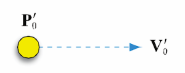
\includegraphics[width=0.35\linewidth]{DR1.png}
    \caption{First order linear projection. Image sourced from \cite{murphy2011believable}}
    \label{fig:dr1}
\end{figure}

%This simple representation of projecting forward is correct if an agent has linear movement and constant velocity. However, agents in games often have complex non-linear movements which will need to be checked for and accommodated. Real world applications of linear dead reckoning also suffer with having to account for unpredictable behaviour e.g. drift due to wind or wheel slippage \cite{chung2001accurate} \cite{ojeda2004experimental}. The techniques used for managing these behaviours are transferable to the problems of dead reckoning networked multiplayer game agents with complex behaviour.

In 1983, with substantial support from the U.S. army, the Defense Advanced Research Projects Agency (DARPA) initiated the Simulator Networking (SIMNET) program which developed dead reckoning techniques to support a virtual world to train soldiers \cite{calvin1993simnet}. Their approach to networking solutions has been incorporated into the Distributed Interactive Simulation (DIS) standard which is now an IEEE standard \cite{dis1998ieee}. It outlines the use of a PDU to help dead reckoning handle complex behaviour \cite{mccarty1994virtual}. It is worth remembering however that DIS was designed for use by a small number of players (less than 50), and the inclusive PDU model can be criticised for holding too much redundant data \cite{henderson2001latency}.
 
Each client maintains a dead reckoned model of itself that corresponds to the model used by other clients to ``see'' its represented agent. The client must regularly check whether the difference between the predicted state calculated with dead reckoning that all clients share and the actual state exceeds a certain threshold. If this is the case, the client is then responsible for generating an updated entity state for the dead reckoning algorithm to apply to the model. Then send that updated state to all clients on the network to learn about the correct state of the agent, to then use to update their own model of that client's agent \cite{calvin1993simnet} \cite{mauve2000keep}. This also happens when a certain amount of time has passed since the last update \cite{mills1992network} (normally 5 seconds).

\begin{figure}[h]
    \centering
    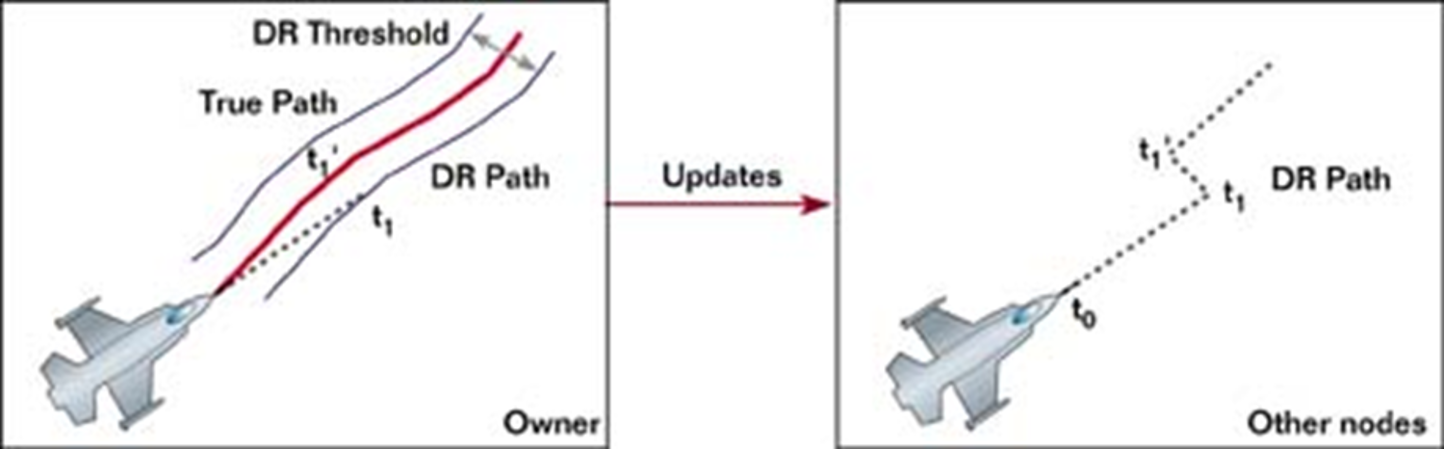
\includegraphics[width=0.9\linewidth]{Threshold1.png}
    \caption{Image sourced from \cite{aronson1997gamasutra}}
    \label{fig:threshold}
\end{figure}

Were this updated information used immediately, the modelled entity would appear to jump (fig. \ref{fig:threshold}). Instead, the dead reckoning algorithm uses interpolation and projective velocity blending \cite{murphy2011believable} to tend towards and eventually reconcile its own dead reckoned model with the updated state information.

\subsection{Implementation} \label{implementation}

Reconciling deviations with projective velocity blending

\begin{figure}[h]
    \centering
    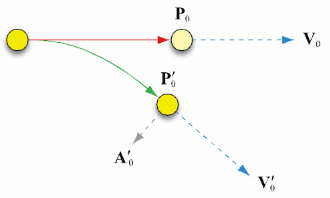
\includegraphics[width=0.7\linewidth]{DR2.png}
    \caption{Upon update, the difference between the simulation shown with $P$ and the actual position shown with $P'$ is observed. Image sourced from \cite{murphy2011believable}.}
    \label{fig:dr2}
\end{figure}

\begin{figure}[h]
    \centering
    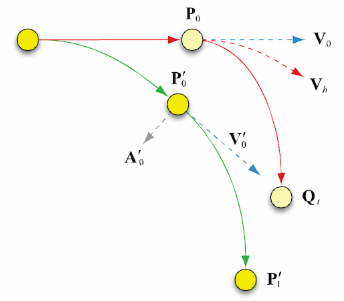
\includegraphics[width=0.7\linewidth]{DR3.png}
    \caption{With interpolation the simulation attempts to reconcile itself with the updated position and motion as discussed in \ref{deadReckoning}. Image sourced from \cite{murphy2011believable}.}
    \label{fig:dr3}
\end{figure}

\begin{align}
        Q_t & = P_0 + VT \\
        Q_t & = {P'_0} + {V'_0} T + \frac{1}{2} {A'_0} T^2 \\
        V_b & = V_0 + ({V'_0} - {V_0}) \Hat{T}  \\
        P_t & = P_0 + {V_b}{T_t} + \frac{1}{2} {A'_0} {T_t^2}  \\
        P'_t & = {P'_0} + {V'_0}{T_t} + \frac{1}{2}{A'_0}{T_t^2}\\
        Q_t & = P_t + ({P'_t} - P_t ) \Hat{T} 
\end{align}

Where $Q_t$ is the dead reckoned position at a specific time $T$ for an entity starting at position $P$, moving at velocity $V$, with acceleration $A$. As shown in fig \ref{fig:dr2} and fig \ref{fig:dr3}, prime ($'$) refers to the actual entity rather than the simulated model. The subscript $0$ refers to the starting value, subscript $t$ is that value at time $T$, and subscript $b$ is the blended model between actual and simulation values. \\
(1) First order linear projection. Shown in fig \ref{fig:dr1} as projecting a velocity over time from a position.\\
(2) Second order projection adds the derivative of acceleration applied according to Newton's laws of motion.\\
(3) Shows a velocity blending model given two velocities. In client-side prediction this would be the simulated velocity and the actual velocity. $V_b$ will tend towards the actual velocity $V'_0$ as delta time $\Hat{T}$ tends towards $1$. \\
(4) Applies the blended velocity value with the simulation's starting position to the second order projection in (2) giving the simulated position at time $T$.\\
(5) Applies the last known actual values to the second order projection in (2) giving the updated projection position at time $T$.\\
(6) Blends these positions tending the simulation towards the updated projection position as delta time $\Hat{T}$ tends towards $1$. \\

\hrulefill

{\sc Threshold based dead reckoning pseudo code}

\hrulefill

\begin{algorithm}
\DontPrintSemicolon % Some LaTeX compilers require you to use \dontprintsemicolon instead
\KwIn{ \\ prediction error threshold: $\eta$ \\ time at which the last position was sent: $t_o$ \\ actual position (at time $t$): $x_t$}
\ForEach{frame (time $t$)}{
  $\Hat{x}_t \gets$ prediction($x_{t_0}, t$);\;
    \If{$|x_t - \Hat{x}_t| > \eta $}{
        send update packet(x_t)\\
        $t_0 \gets t$\;
    }
}
\caption{A client predicts the position of their own agent for the current frame based on the last sent update information. If the prediction error is larger than the threshold ${\eta}$ then an update packet is sent to the network and the simulation resets itself.}
\label{algo:pseudo}
\end{algorithm}

\subsection{Interest modelling} \label{interestModelling}

The shortcomings of estimating a game agent's behaviour based solely upon motion dynamics are already recognised and attempts to address these problems with further information have been somewhat explored. The \textit{Donnybrook} protocol \cite{bharambe2008donnybrook} looks to increase the delay between packets up to seconds by leveraging user limitations to use bandwidth preferentially on the information most important to the player's \textit{interest sets}. Similarly, Amir Yahyavi \textit{et al} successfully use identified points of interest to influence their dead reckoning algorithm, improving the accuracy by up to 30\% over traditional dead reckoning techniques \cite{yahyavi2011antreckoning}.

Yahyavi \textit{et al} propose the use of \textit{attraction forces}, derived from the player state and nearby points of interest, to be factored into the dead reckoning calculation alongside the current acceleration. The example that they often cite states that a player controlling an entity with reduced health will most likely move towards a health pack if there is one in sight. However, their method titled \textit{AntReckoning} must decide on the attraction forces of each point of interest, to build a \textit{pheromone map}. AntReckoning's weakness is great complexity as every change in the game state affects nearby attraction forces. Also the reliability of AntReckoning can be disputed as different players may have differing goals, but the increase in accuracy reported is excellent. This can also be used to influence the path finding algorithms of non playable characters (NPCs) controlled by an artificial intelligence to direct them towards popular parts of the level \cite{yahyavi2013interest} \cite{yahyavi2013towards}. While this shows an interesting application of utilising level information, the behaviour of NPCs is beyond the scope and focus of this project.

The merit of Amir Yahyavi \textit{et al}'s work \cite{yahyavi2011antreckoning} \cite{yahyavi2013interest} recognising and proposing solutions to the problems of solely using traditional dead reckoning methods in games with client-side prediction is acknowledged, and an inspiration for this project.

\subsection{Adapting the acceptance threshold} \label{adaptingThreshold}

As shown in algorithm \ref{algo:pseudo}, the condition that prompts a network update is that the difference in position between a client's own entity and the representation of that entity used by the network differ by more than a threshold amount. This amount can be visualised as an acceptance radius around the dead reckoned position as shown in fig \ref{fig:threshold}. Generally, dead reckoning algorithms employ a fixed threshold \cite{cai1999auto}. Related work that investigates changing this threshold amount depending on game state conditions decide the variance by considering the individual peer to peer relationships such as the distance between the agents. This \textit{relevance filtering} is reliant upon a \textit{radius of interest} \cite{rak1996evaluation}. The reasoning given is that distant agents are not likely to interact with each other so accuracy is not particularly important \cite{cai1999auto} \cite{jaya2016combining}.

This paper acknowledges this method's effectiveness in specific situations to reduce network updates. But, given the often edge to edge viewing range prevalent in many game first-person shooter levels \cite{toby2014tobyscs} \cite{ziervogel2014nag} \cite{cod2018wikibo4}, this paper argues against its use in a general approach to improving client-side prediction in first-person shooter games.

To allow for edge to edge sight lines and the prevalent long range weapons available for use in first-person shooter games, we can consider filtering for entities that are within that player’s potential field of sight \cite{cronin2001distributed}. However, this requires previous knowledge of all entity positions therefore a two pass approach would be needed to determine which entities would be affected by a state change, and then to update those clients. Also, care must be taken as even when entities are out of sight of each other, dead reckoning may predict a behaviour which results in the entities being revealed and the integrity of the game state will be compromised.

Roberts \textit{et al} propose that network update time should be factored into deciding the threshold limit value. Network limitations when presented with a large amount of packets may result in inconsistency for which additional updates are needed to rectify \cite{roberts2008bounding}. This shortcoming in a networked application is an important consideration. However, given the local prediction methods of this project, fall outside of this study. Were future work to lead to a networked experiment, and given the proposed increase in packets sent at critical junctures, the relevance of considering network shortfalls when calculating a dynamically changing threshold will be crucial.

%\subsection{Doppelg\"{a}ngers} \label{doppelgangers}

%\textit{Doppelg\"{a}ngers} offer a promising alternative that will adhere to the game's rules and avoid impossible behaviour. Jeffrey Pang \textit{et al} discuss populating a client's game state representation with computer-controlled players known as \textit{bots}. Updates prompted by a threshold based system similar to that outlined in algorithm \ref{algo:pseudo} will contain \textit{guidance} for the artificial intelligence (AI) to rectify and better replicate the relevant representation \cite{pang2007scaling} \cite{bharambe2008donnybrook}. As most first-person shooter games contain AI routines for single player modes, much of the work needed to guide a bot around a level has been done. Problems will occur if a bot representation decides that it will perform an action such as shoot at an enemy, whereas the actual behaviour does not. Questions arise such as should the bot then fire ``blanks'', and consideration must be given as to whether that action may inadvertently alert enemies to that entity's position? This approach shows considerable potential in providing possible and realistic representations of other clients' behaviours, but relies heavily upon accurately portraying and dynamically adjusting the bot's AI behaviour model. To configure the AI behaviour, neural networks can be trained and used to predict changes of the entity velocity \cite{mccoy2007multistep}. Jeffrey Pang \textit{et al} propose that a blending between an AI bot for non-critical behaviour e.g. outside of the client's focus, and conventional dead reckoning state updates for representations of entities within the player's focus will provide a satisfying result \cite{pang2007scaling}.

%This paper argues in favour of bot representations as both a method to decrease the frequency of network updates, and as a tool to extrapolate future behaviours. But, also acknowledges its dependency upon accurate player modelling techniques. Player modelling is an ongoing study in the field of games. Since the focus of this work is on dead reckoning in client-side prediction we omit further details about AI modelling player behaviour, although we strongly consider this as future work in the field of client-side prediction.

\section{Discussion} \label{discussion}

The two part purpose of client-side prediction is to maintain an up to date game state for clients in the case of late or lost packets, and to use prediction algorithms to reduce required network updates. While the simplest dead reckoning algorithm provides a linear vector approximation based on velocity, we have described how interpolation and projective velocity blending can be used to smooth trajectories between state updates tending towards the correct representation.

Benjamin Kuipars states that the difficulty of a dead reckoning task should vary according to the number of turns in the route, while the error rate and magnitude should vary according to the complexity of the route \cite{kuipers1978modeling}. So, we can infer that likewise when considering complex paths with many turns, to expect a larger error rate.

It is a fundamental requirement for believable games that the state transitions and corrections are smooth and believable, shown in figures as a curve tending towards the target rather than a jump. These curves are shown to be accurate when inferred from polynomial modelling based on the Lagrange or Taylor series \cite{hanawa2006proposal}. But require multiple states from which to extrapolate an approximation. Packet loss can be greatly detrimental to this approach. Small sample sizes combined with potentially erratic movement of game players will likely produce unlikely results. A solution would be to provide back up copies of previous states in each PDU to restore missing information. A technique already employed in Quake where the last three commands are also sent in each packet to compensate for lost packets \cite{cronin2001distributed}. James M. Van Verth and Lars M. Bishop provide a method to sample and project cubic bezier spline curves \cite{van2008essential} but these are shown to be slightly less accurate than the velocity blending technique shown above proposed by Curtiss Murphy \cite{murphy2011believable}. 

Dead reckoning is an \textit{optimistic algorithm}. It assumes it is correct  and when it is not, it must adjust itself. It is apparent that the blending of this adjustment may result in compromising behaviour. Demonstrated in first-person shooter games as appearing to other players in a vulnerable position outside of cover, or moving through an impenetrable area as defined by the game's movement rules. Consider the velocity blending method shown in fig \ref{fig:dr3} and (6). A player could turn instantaneously and the algorithm would apply unrealistic acceleration to reconcile the position change \cite{bernier2001latency}. Large inconsistencies due to extremely late or lost updates may lead to repairs requiring a state rollback which will cause more drastic position jumps \cite{cronin2002efficient}. The resulting movement shown by the simulation path in fig \ref{fig:dr3} may also fall outside the rules of the game. Either passing through untraversable locations such as through walls or over gaps, or into unlikely locations according to the game's rules such as into a vulnerable position outside of cover. Many networked multiplayer first-person shooter games suffer from criticism because of this. Players can feel unfairly treated and forums discussing these issues become very popular with many thousands of views \cite{rout2013youtube} \cite{gkac2014gamefaqs} \cite{drift0r2013youtube} \cite{solaire2016reddit} \cite{ss2018reddit} \cite{hp2015bungie}.

The de facto method of dead reckoning entities' behaviours is a distributed approach that does not necessarily require a centralised server. Using a distributed approach for a distributed virtual environments (DVEs) can avoid the problems of centralised systems such as an increased latency and a single-point-of-failure \cite{mauve2000keep}. However, having a dedicated central authoritative server (or a single client nominated as such) means that if a client simulates different results than the server, the server’s authority can forcefully correct the client’s simulation \cite{bernier2001latency}. Similarly, in \ref{deadReckoning} we mention network latency not succeeding due to state conflict, where simultaneous conflicting actions are performed by multiple clients. In this case, the authoritative server, the client acting as such, or the game itself, must decide which state is the ``correct'' state and update all conflicting clients with that decision. Games will often invoke a small delay before critical moments e.g. a death animation, to allow conflicting states to resolve themselves before committing to a particular irreversible state. With this delay, the game can rollback to the correct state without the user experiencing a jarring state change \cite{mauve2000keep}.

Client-side prediction is necessary to compensate for latency and reduce the impact of packet loss upon the user experience. Correctly leveraging the prediction method can decrease packet loss or lateness caused by network congestion by relying upon correctly predicting a player's future behaviour rather than updating the behaviour with many packet updates.

\subsection{Representing level data} \label{representingLevelData}

This project explores whether experiential trend information regarding an agent's position within the level can be used to more critically evaluate when to send update packets for a more efficient client-side prediction method. As such, effectively storing and evaluating spatial information about the changes in motion of agents moving around a level is paramount. 

\begin{figure}[h]
    \centering
    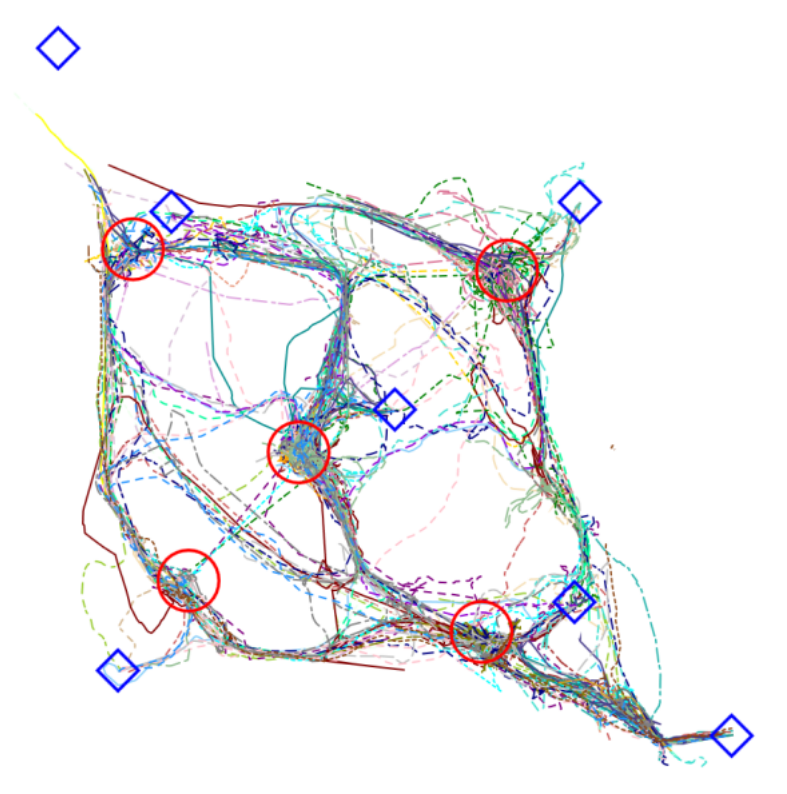
\includegraphics[width=0.9\linewidth]{Heatmap3.png}
    \caption{980 player trajectories from the ``Arathi Basin'' battleground from the game \textit{World of Warcraft}. Circles show strategic points and diamonds show graveyards which are used as spawn locations. Image sourced from \cite{miller2009avatar}.}
    \label{fig:hm3}
\end{figure}

\begin{figure}[h]
    \centering
    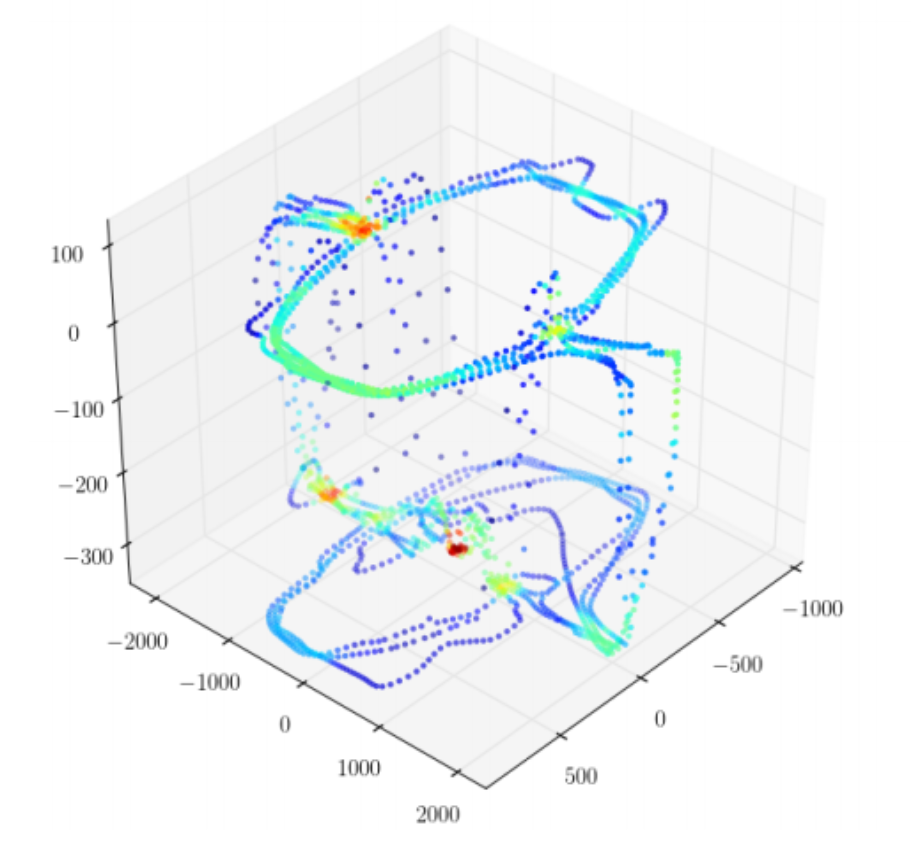
\includegraphics[width=0.9\linewidth]{heatmap4.png}
    \caption{Representing spatial clustering and player movement in the ``Gael'' map from the game \textit{Unreal Tournament 2003} showing clustering behaviour. Image sourced from \cite{bauckhage2014beyond}.}
    \label{fig:hm2}
\end{figure}

A heat map is a visual reflection of a statistical model \cite{wilkinson2009history} used often in games to graphically represent spatial analytics of player data with colours, overlayed upon a traditional map of the level (see fig \ref{fig:hm2}). They are a tool to help extract patterns and knowledge which can be used to detect outlying data \cite{drachen2013spatial} (Apparent in fig \ref{fig:hm3} as single paths travelling perpendicular to the trend). To this end, as a tool, it meets our needs perfectly. Where interest modelling seeks to better predict a single entity's interest, our proposed method outlines a broadly applicable use of movement trend information in a level to produce a more reliable prediction model, without significantly affecting the accuracy of the simulation.

Unlike the path visualisation as shown in fig \ref{fig:hm2}, the direction of motion must be asymmetric. Consider that a player may jump down from a platform but be unable to get back onto it \cite{bauckhage2014beyond}. Consideration must also be given to symmetrical paths with equal footfall. The proposed method relies on the idea that a perpendicular vector to the trend must be realised as countering the norm. This may not be apparent where opposite paths accumulate to a zero score.

Finally, the map must be partitioned in such a way that the information is relevant. Large size cell partitioning can disproportionately accumulate several critical positions within \cite{steed2003partitioning}. Care must be taken to choose an effective grid size before formatting it into a state that the client-side prediction algorithms can effectively use. Heat maps can be represented within a program as either a two-dimensional data structure for spatial representations like that of fig~\ref{fig:hm3}, or a three-dimensional data structure for those like fig~\ref{fig:hm2}.

Heat maps, or data structure equivalences, are used in games for training bots to behave more realistically and improve map design during development \cite{bauckhage2014beyond} but to the best of our knowledge have not been applied to alter prediction algorithms' values or alter the network update frequency.

\section{Evaluation} \label{evaluation}

The literature shows a broad approach to the trade off between network latency implications and accurately representing every entity's behaviour. Finding the balance between excessive network congestion and maintaining an accurate representation of the game state for all clients is a challenge faced by all networked multiplayer games. Dead reckoning methods are highly effective, but are solely concerned with an entity's predictable motion. Derivatives such as AntReckoning attempt to model a player's likely intention, although when an assumption of a player's actions are incorrectly predicted, rolling back the game state can be a jarring and detrimental experience to the users.

Where network latency would cause the received data to be slightly behind, client-side prediction algorithms can increase the interval of packet updates and negate the effects of network latency at the cost of representation consistency. In the case of lost packets resulting in no update data for that agent, client-side prediction methods can be used to simulate an agent's behaviour reducing the impact of a network transmission delay. When used effectively this can help to synchronise the game state across all clients.

Related work seeks to minimise the number of required updates and maintain an up to date game state for all clients despite network latency and jitter. However, research into influencing the prediction methods with level specific data is lacking. Altering the threshold has been explored before, as has location evaluation in the form of interest modelling or by area of interest, but to this paper's knowledge no study has combined altering this threshold amount by use of a predetermined vector map showing motion trends.

Unfavourable reactions from users about poor game state management show the importance of finding an effective solution to minimising client-side prediction error, and forms the motivation for this project. While the focus of this project is on first-person shooter games, any improvement to client-side prediction methods will be applicable to other networked multiplayer games that rely upon client-side prediction and dead reckoning to maintain an up to date state representation for all clients. This includes sports or racing games (consider in a racing game, a player will slow down before a corner \cite{larsson2016movement}), given that there has been opportunity to collect player motion information for the level beforehand.

\section{Proposed solution} \label{proposedsolution}

In light of the literature review, it is apparent that attempts to improve client-side prediction regarding the use of dead reckoning concedes an increased overhead with the likes of interest modelling (\ref{interestModelling}) or relevance filtering (\ref{adaptingThreshold}). Motivated by the lack of any approach to a predetermined optimisation model, this project focuses upon building up a level layout specific data set of velocity trends with which to dynamically adjust the frequency of packet updates.

This project encourages reducing the acceptance threshold of the algorithm, increasing the rate of network updates to be sent, at locations where the agent's motion is not compliant with the derived trend for the grid square that it occupies. This will preempt a likely change in motion and enable a prediction model to see that change earlier than if waiting for a constant acceptance threshold to be exceeded. This is balanced by increasing the acceptance threshold of the algorithm where the agent's motion is compliant with the location's derived trend, under the presumption that predictable movement will follow predictable movement. This proposal considers that a packet update prompted by a large threshold will require the prediction model to undergo a greater distance reconciliation than that prompted by a small threshold. So, as the error threshold changes, so must the blend time that is used to reconcile the current prediction model with any updated information. As the threshold increases, the time given to reconcile any deviation should decrease, so this relationship is inversely proportionate.

This paper names this method \textit{level experiential dead reckoning} (led reckoning). The proposed led reckoning method mirrors the dead reckoning method with the following amendments:

\begin{align}
        \text{1) Correlation-} & \text{based threshold adjustment} \nonumber \\
        \nonumber \\
        C & = |{V_b} \cdot {V_p}| \label{eq:correlation} \\
        \nonumber \\
        \eta_p & = {\eta_{min}} + C ({\eta_{max}} - {\eta_{min}}) \label{eq:threshold} \\
        \nonumber \\
        \text{2) Threshold-b} & \text{ased blend time adjustment} \nonumber \\
        \nonumber \\
        B_t & = \frac{K}{\eta_p} \label{eq:blendtime} \\
        Q_t & = P_t + \frac{\Hat{T}} {B_t} ({P'_t} - P_t ) \label{eq:motion}
        \\ \nonumber
\end{align}

Where $V_p$ is the velocity trend at a position $P$ in the level. $C$ is the correlation score between the motion and the trend. $\eta_p$ is the error threshold to be used at position $P$. $\eta_{min}$ is the constant minimum threshold allowed by the game. $\eta_{max}$ is the constant maximum threshold allowed by the game. $B_t$ is the blend time for the prediction model to reconcile with the the any updated packet information. $K$ is a constant coefficient for the inversely proportionate relationship between the blend time and the threshold.
\\ \\
(\ref{eq:correlation}) Declares the absolute value of the dot product of the blended velocity model found with (3), and the direction trend for the entity's position in the level as the correlation score between the simulation and the data trend. \\
(\ref{eq:threshold}) Uses the correlation score $C$ as a blend value, to return a threshold amount for the entity at position $P$. The returned threshold amount is blended between $\eta_{min}$ and $\eta_{max}$ by the $0 - 1$ correlation score $C$. \\
(\ref{eq:blendtime}) Calculates an informed blend time value $B_t$ that is inversely proportionate to the threshold. The coefficient $K$ is a multiplier to return a usable blend time value. \\
(\ref{eq:motion}) Takes the projective velocity blending equation (6) and divides $\Hat{T}$ by the adjusted blend time so that $Q_t$ tends towards $P'_t$ as $\Hat{T}$ tends towards $B_t$.

\section{Research methodology} \label{researchmethodology}

The research question addressed in this project is: how can client-side prediction in networked multiplayer first-person shooter games that use dead reckoning be improved? The hypotheses drawn from this question are listed in table~\ref{table:hypothesis}.

This project's hypotheses is tested by comparing two distinct client-side prediction simulations of a path. One using a traditional dead reckoning method, and another using this paper's proposed led reckoning method. The fields for comparison will be the mean average number of packet updates prompted per second, and the mean average distance of the prediction model position from the path's actual position measured every frame. Any variance in the number of packet updates are discussed considering any variance in accuracy of the prediction simulations.

\subsection{Hypotheses} \label{hypothesis}

\begin{table*}[t]
	\centering
	\caption{Hypotheses}
	\label{table:hypothesis}
	\def\arraystretch{1.5}
	\begin{tabular}{|c|p{7.1cm}|p{7.1cm}|p{1.5cm}|}
		\hline
		& \textbf{Hypothesis}& \textbf{Null Hypothesis} & \textbf{Data Source} \\ \hline
		%
		1 & Using the player's correlation with location specific motion trends derived from experiential data to adjust the dead reckoning error threshold responsible for prompting packet updates and the reconciliation blend time will result in a fewer number of required packet updates than that with a constant error threshold.
		& Using the player's correlation with location specific motion trends derived from experiential data to adjust the dead reckoning error threshold responsible for prompting packet updates and the reconciliation blend time will result in a greater number of required packet updates than that with a constant error threshold.
		& Replay data experiment results \\ \hline
		%
		2 & Using the player's correlation with location specific motion trends derived from experiential data to adjust the dead reckoning error threshold responsible for prompting packet updates and the reconciliation blend time will result in a client-side prediction model that is not significantly less accurate than that with a constant error threshold.
		& Using the player's correlation with location specific motion trends derived from experiential data to adjust the dead reckoning error threshold responsible for prompting packet updates and the reconciliation blend time will result in a client-side prediction model that is significantly less accurate than that with a constant error threshold.
		& Replay data experiment results \\ \hline
	\end{tabular}
\end{table*}

Table \ref{table:hypothesis} shows the hypotheses that are tested in this experiment. Equations (7) -- (10) show the implementation of the hypotheses by amending the dead reckoning implementation as described in \ref{implementation}. Testing these hypotheses requires comparing the results of a standard dead reckoning implementation and the same algorithm amended to include derived movement trend data to alter the algorithm's threshold value and the reconciliation blend time. As this is a comparison of client-side prediction algorithms, the experiment acts as if there is zero network latency. Jitter and packet loss simulations will add unnecessary complication to the algorithms where this project is focused on the accuracy of the prediction model and the number of requested packet updates.

\subsection{Data collection} \label{datacollection}

To validate the proposed algorithms and seek confirmation of the hypotheses, this project uses movement data from an existing game. The design implications of attempting to recreate a believable online multiplayer scenario as a test bed are unnecessary when these scenarios are available already. As the data must reflect an online multiplayer game player's movement, this project evaluates replays of existing online games. This removes any participant bias that recruiting test subjects may incur, and any complexities in attempting to create an online multiplayer game scenario where subjects are required to behave as if they are actually playing an online multiplayer game.

This project uses the game Counter-Strike: Global Offensive\footnote[1]{Available: \url{https://store.steampowered.com/app/730/CounterStrike_Global_Offensive/}} (CS:GO) as a test bed. CS:GO is an online multiplayer first-person shooter game developed by Hidden Path Entertainment and Valve Corporation. It is a ten player, two team game, where each of the two five-member teams compete over many rounds to complete their team's objective. Due to CS:GO's popularity as an eSport, there is an abundance of tournament replay data available online. The implication of collecting high profile competitive eSports movement data is that the players being examined will have an extremely high skill level in the game. As such, the author considers the movement choices that these player's make to be the \textit{best} choices given the player's situation. This eliminates any concern over non objective orientated movement contaminating the trend data. The player's movement can be thought of as a direct result of the player's consideration of their current objective from their current location. While objectives will often include the elimination of enemy players nearby, sustained objectives will become apparent by the trends shown from averaging many players' movements. These common objectives may be a goal of the game, or a common enemy position. It is the intent of this experiment to be indifferent to the cause of a trend's apparent goal, but to promote a method for identifying probable paths, unconcerned whether moving towards a potential objective, or away from an undesirable area.

Among the many levels available, \textit{Inferno} (see fig~\ref{fig:inferno}) was chosen to experiment upon. Inferno has very little verticality in its design as opposed to other levels where different rooms and corridors are placed above and below each other. By testing the hypotheses on such a level, the results can be viewed in a two dimensional visualisation such as shown in fig~\ref{fig:hm2} without introducing a height vector as shown in fig~\ref{fig:hm2}. As each $(X, Y)$ coordinate relates to a single specific location in the level (without having to factor in a $Z$ \textit{floor} location), the velocity trend data structure can be simplified to a two dimensional array to reduce complexity yet still serve as a proof of concept. The method proposed can be expanded to a three dimensional data structure to be used in the same way and serves as future work in the field.

\begin{figure}[h]
    \centering
    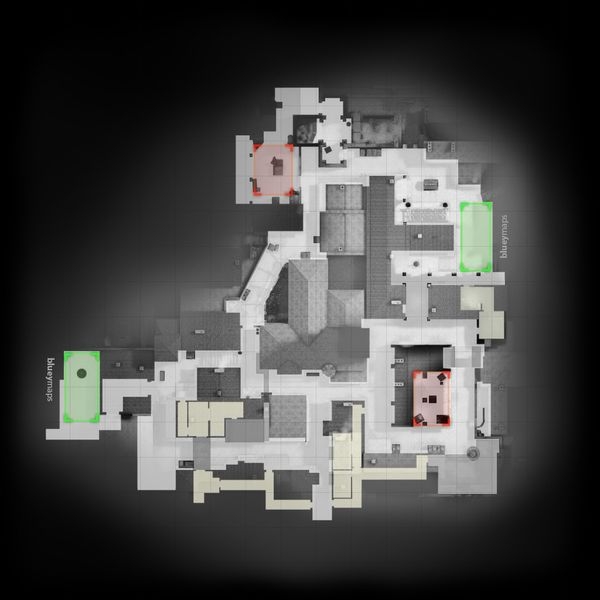
\includegraphics[width=1.0\linewidth]{_InfernoMapImage.jpg}
    \caption{The Inferno map from CS:GO}
    \label{fig:inferno}
\end{figure}

CS:GO replay files are in the form of \textit{video game demo} (DEM) files. This format has been developed by Valve to hold the game replay data to be opened within the game to view the match. DEM files can be found freely available online most prominently in eSports reporting communities. This project uses the reputable \textit{GosuGamers}\footnote[2]{Available: \url{https://www.gosugamers.net/counterstrike/demos}} as the source for the DEM files used. GosuGamers is an online reporting website for many eSports games, including CS:GO, League of Legends, DotA 2, and Hearthstone.

161 Inferno DEM files are available from competitive tournaments from 2014 to 2016. However, the DEM files occasionally contain more than the fixed amount of ten players allowed. In competitive scenarios these extra player names represent team coaches and tournament adjudicators so the files are first parsed into individual players by in game player names. These non-players are identified as comparatively small amounts of information relative to the rest and are removed from the data as they are not valid players moving according to the game's objectives.

From the stream of each player's frame data, a player death and restart event or the end of the game round can deduced by comparing the position described in each frame to the previous, and looking for changes in position that exceed the game's movement rules. Each player's information identified in the DEM file is parsed with this method resulting in many individual paths and saved to an individual comma separated values (CSV) file, where each row holds the player's information for a game frame and the row number pertains to the frame number. The project uses CSV files here as .NET framework is efficient at reading and processing a file stream line by line similar to the frame by frame process of games, and applicable to the task of sequentially recreating a player path. Finally, due to CS:GO gameplay incurring a five second introductory warm up round with no objective, all player paths less than five seconds in length are discarded as a safeguard against including non-typical in game behaviour.

This process resulted in 43,305 player paths. To give more context to this amount of data, the total size of the CSV files is 7.65GB or approximately 85,000,000 frames of data. As the game records at 60 frames per second, this is greater than 1,400,000 seconds (approximately 16.5 days of gameplay frame data). This shows a mean average time of approximately 33 seconds per path. These numbers are approximate due to CSV header file space and differing CSV entry lengths and are purely anecdotal and contextual.

\section{Software development}

To parse and simulate client-side prediction algorithms upon the DEM files, a program written in C\# .NET framework using Microsoft Visual Studio Community 2017 has been used due to the frameworks efficiency in reading CSV files as a stream of data, and the developer's familiarity with the tools. C\# .NET framework is a popular and well supported commercial framework that has a lot of functionality that this project needs so that multiple additional software libraries are not needed. .NET framework's Stopwatch class was used for benchmarking when optimising the source code, and the MessageBox class is used for explicit feedback of values and errors. A WinForms graphical user interface (GUI) has been used to aid easily selecting files which is required due to the large number of CSV files representing individual paths required. The GUI can also display graphics necessary to visualise the player paths and their relationship to the prediction algorithms' paths. WinForms was chosen to aid and speed up development as a specialised tool was not needed.

Parsing the DEM files was achieved using the package \textit{DemoInfo} by EHVAG\footnote[3]{Available: \url{https://github.com/StatsHelix/demoinfo}}. This is a popular DEM file parsing library in the CS:GO community, and is published under the open source MIT license\footnote[4]{Available: \url{https://github.com/StatsHelix/demoinfo/blob/master/License.txt}}. Trello\footnote[5]{Available: \url{https://trello.com/}} was used as an online task management tool due to its ease of use and lightweight approach in describing the multiple processing tasks required by the program. To analyse the results RStudio\footnote[6]{Available: \url{https://www.rstudio.com/}} was used as a reputable statistical analysis tool.

\subsection{Software development life cycle} \label{lifecycle}

Starting with the data set and then developing a program to parse, process, and experiment upon it has required an iterative agile approach to development due to multiple user stories and to allow for changing requirements. Initially, development began with a series of short one week sprints; each concerned with a different step of the parsing process. Firstly, the program had to be able to read information from the DEM file and parse that information into a usable format. As outlined in \ref{datacollection}, the data was next screened for irrelevant player names beyond the number of players that the game allows. By parsing the DEM files into separate player files with an explicit naming convention of \textit{\url{game_name.player_number.CSV}} and incrementing the player number upon the discovery of a new name in the replay file, it was a straightforward process to manually remove any additional player files that did not belong. All of which were obvious as being several orders of magnitude smaller in size than the the actual players. The CSV files were structured so that each row sequentially pertained to a frame from the game, and each column contains a piece of game information relevant to the player character in the game at that frame. The developer chose to include all available data in these files, aware that information seeming trivial at this stage may be required if future work chose to explore the player's behaviour in greater depth. These comprise of:
\begin{itemize}
    \item Name
    \item Team
    \item Position
    \item Velocity
    \item View direction
    \item Health
    \item Armour
    \item Active weapon name
    \item If the player is ducking
    \item If the player has a helmet equipped
    \item If the player is carrying a defuse kit
\end{itemize}

Each player file was then read line by line as a stream by the program to discover where individual paths started and ended. This was detected by a distance check between the current position in game, and the previously read line's position. The end of a path would be apparent as a change in position far exceeding any possible movement. Lastly, these were screened in size to be longer than 5 seconds in duration as justified in \ref{datacollection}, before being saved with the naming convention \textit{\url{game_name.player_number.path_number.CSV}} to form the viable data set.

With the raw data sanitised and processed, the velocity trend generation method was then designed. Firstly, an appropriate level of detail for the level partitioning was decided at 100 subdivisions on each axis. As described in \ref{representingLevelData} this is visibly sufficient for Inferno to not accumulate several critical positions within one area. A $100 \times 100$ data structure is declared and populated with the velocity values from every frame of every path that is chosen to form the trend data. The velocity values are accumulated and then averaged for the mean value. It is with this process that the iterative agile philosophy became invaluable. The first design of this process, although effective, required several hours to complete. By iterating over the design and testing, this process was able to be significantly optimised. Further detail of this process can be found in appendix \ref{databaseapproach}.

At this stage, development sprints changed to iterations of design, development, and testing the implementation of the standard dead reckoning client-side prediction algorithm that would sequentially read each line of a player path CSV file as if it were reading game data frame by frame in an actual application. This algorithm will form the base class of this project's proposed method and will be identical in all functionality save the amendments proposed in \ref{proposedsolution}. To fine tune the dead reckoning variables such as error threshold and reconciliation blend time (see \ref{implementation}) a visualiser for the GUI was used alongside an analysis report outputted after each path was used to execute a simulation. Appropriate values were found through iterative assessment that a predicted path's position values are satisfactorily similar to the actual path both in analysis of the deviation and visually in the GUI, and that the number of required packet updates were infrequent enough to allow improvement. Whilst acknowledging the potential improvements of correctly balancing these values, the author proposes that as any imperfect base values are shared, they are inconsequential to the comparative improvements shown. Conclusively perfecting these values falls beyond the focus of this study.

\begin{figure*}
    \centering
    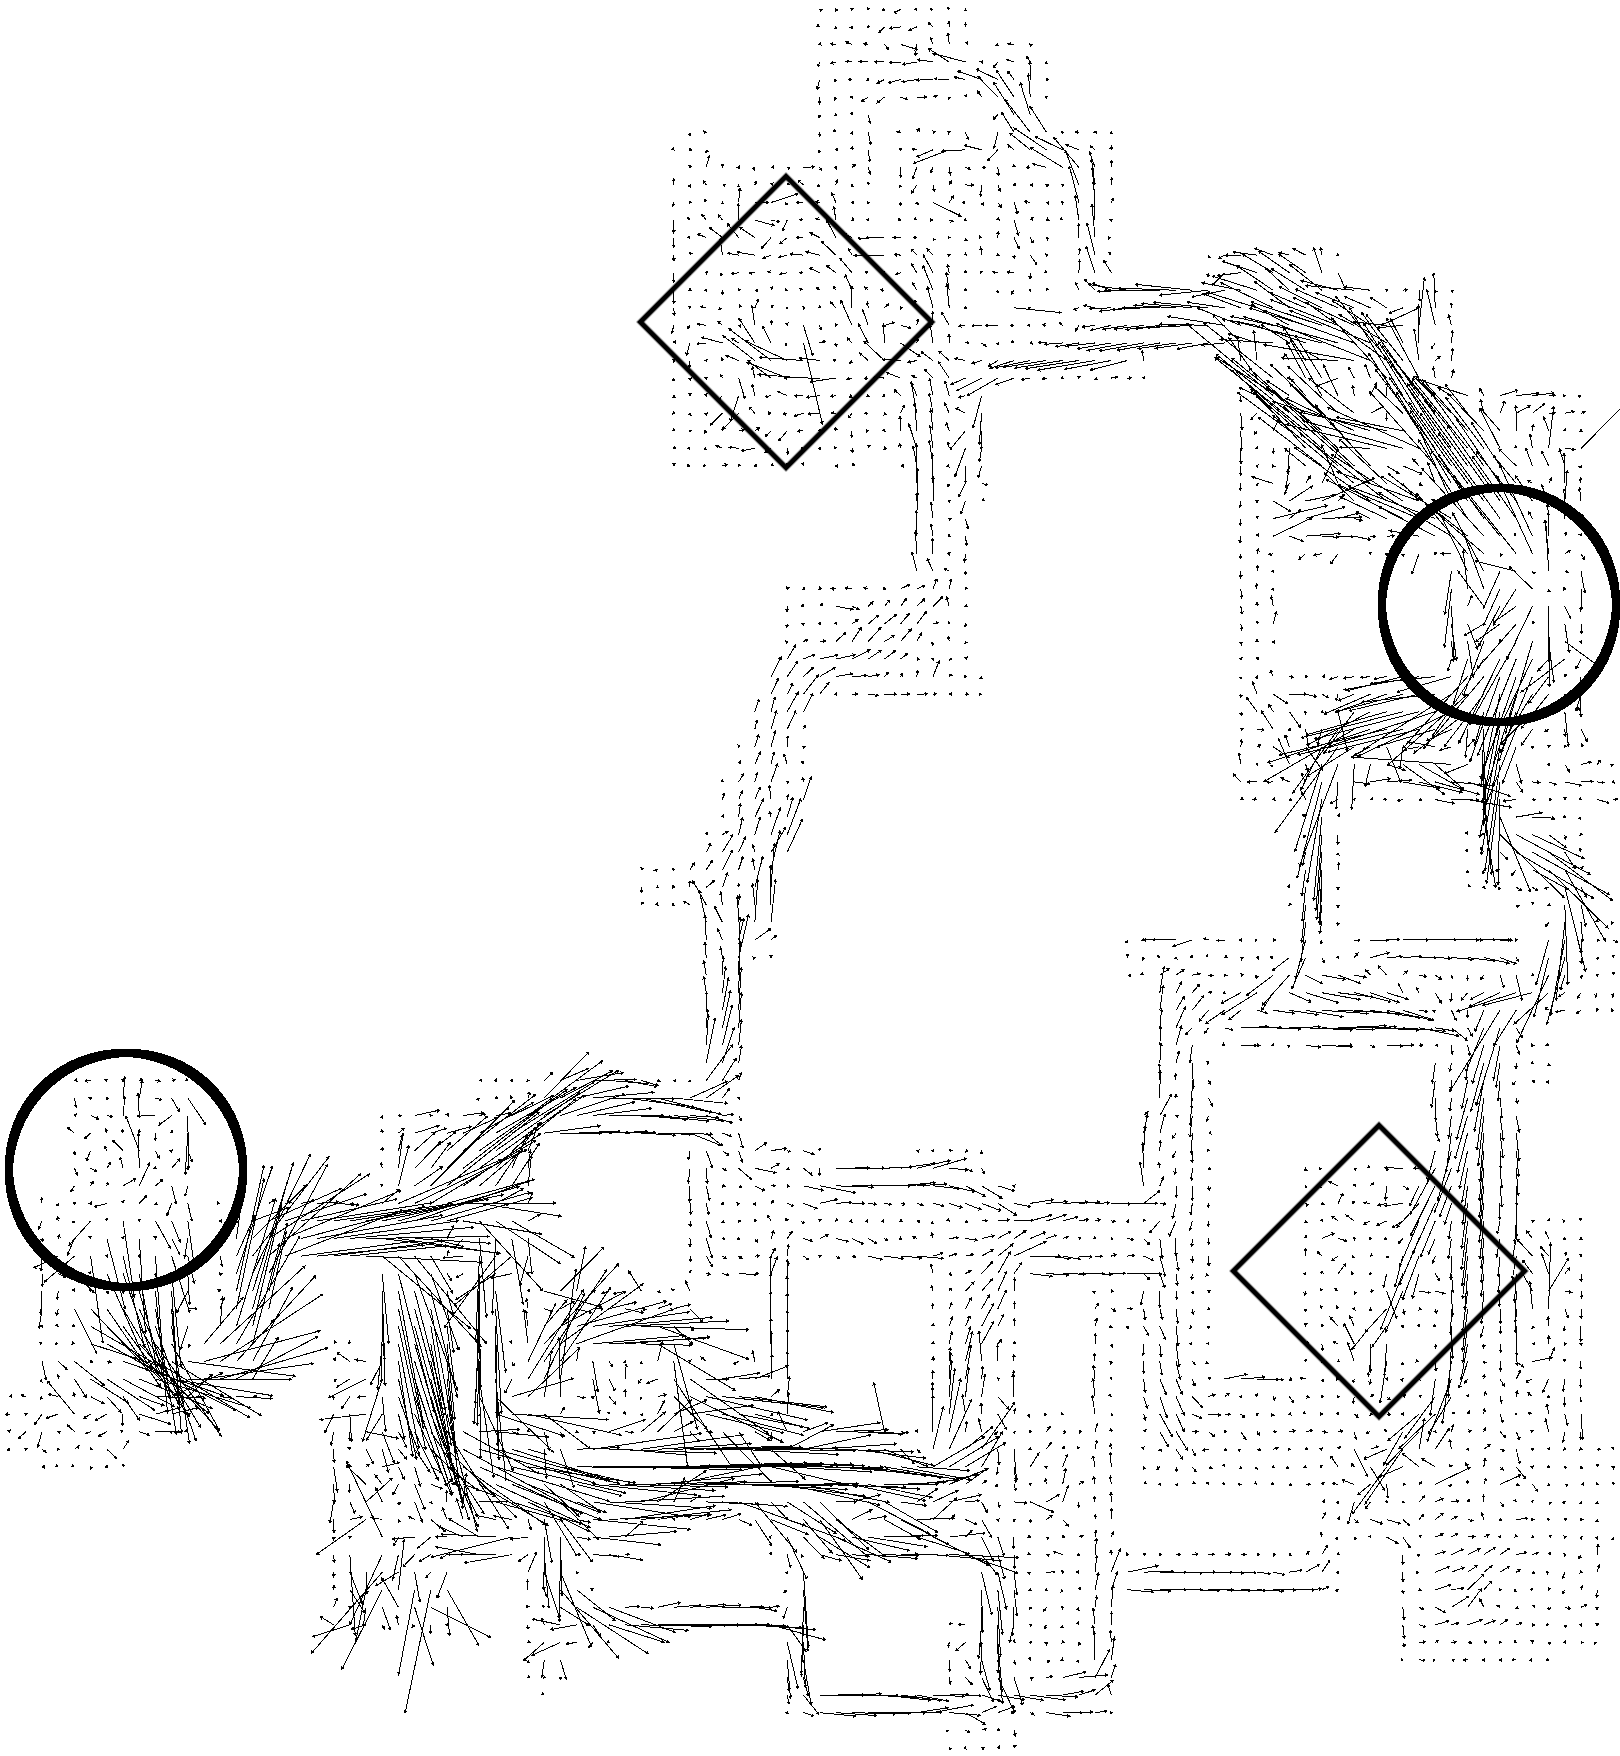
\includegraphics[width=\textwidth,height=1.084\textwidth]{TrendMapBoth.png}
    \caption{The all inclusive trend map showing trends zeroing towards the centre of the map where opposite paths converge. Team start locations are shown by circles, and game objectives are shown by diamonds. Trend maps refined by team showing a more thorough coverage are shown in fig~\ref{fig:trendmap_t} and fig~\ref{fig:trendmap_ct}.}
    \label{fig:trendmapboth}
\end{figure*}

\begin{figure}[h]
    \centering
    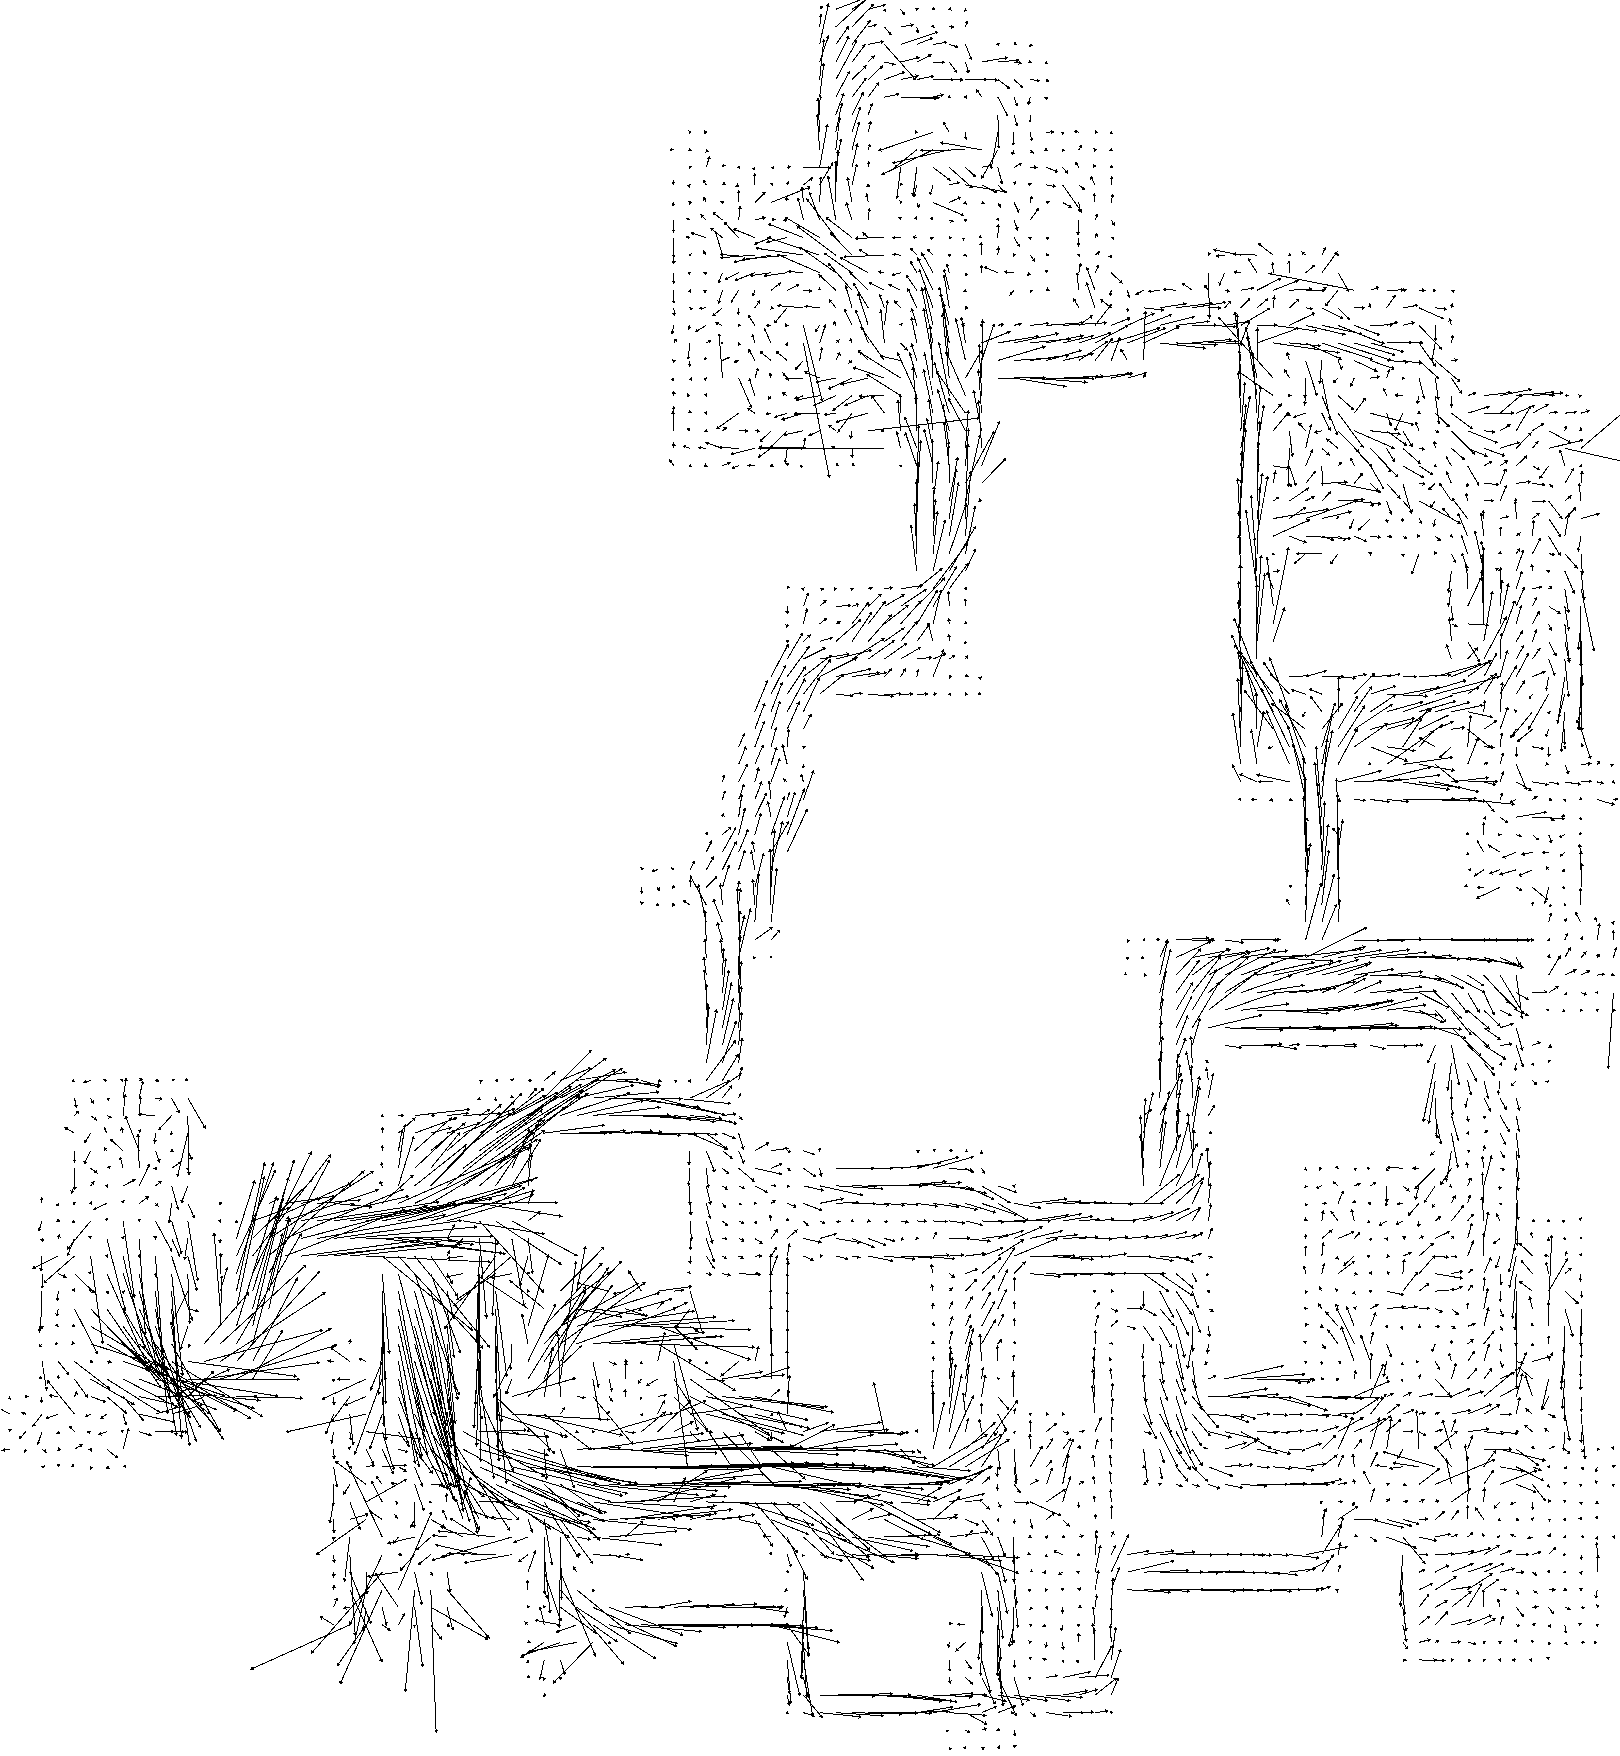
\includegraphics[width=\linewidth]{TrendMapT.png}
    \caption{The \textit{``Terrorist''} team trend map showing visually stronger trends than the all inclusive trend map shown in fig~\ref{fig:trendmapboth} where the opposing teams meet.}
    \label{fig:trendmap_t}
\end{figure}

\begin{figure}[h]
    \centering
    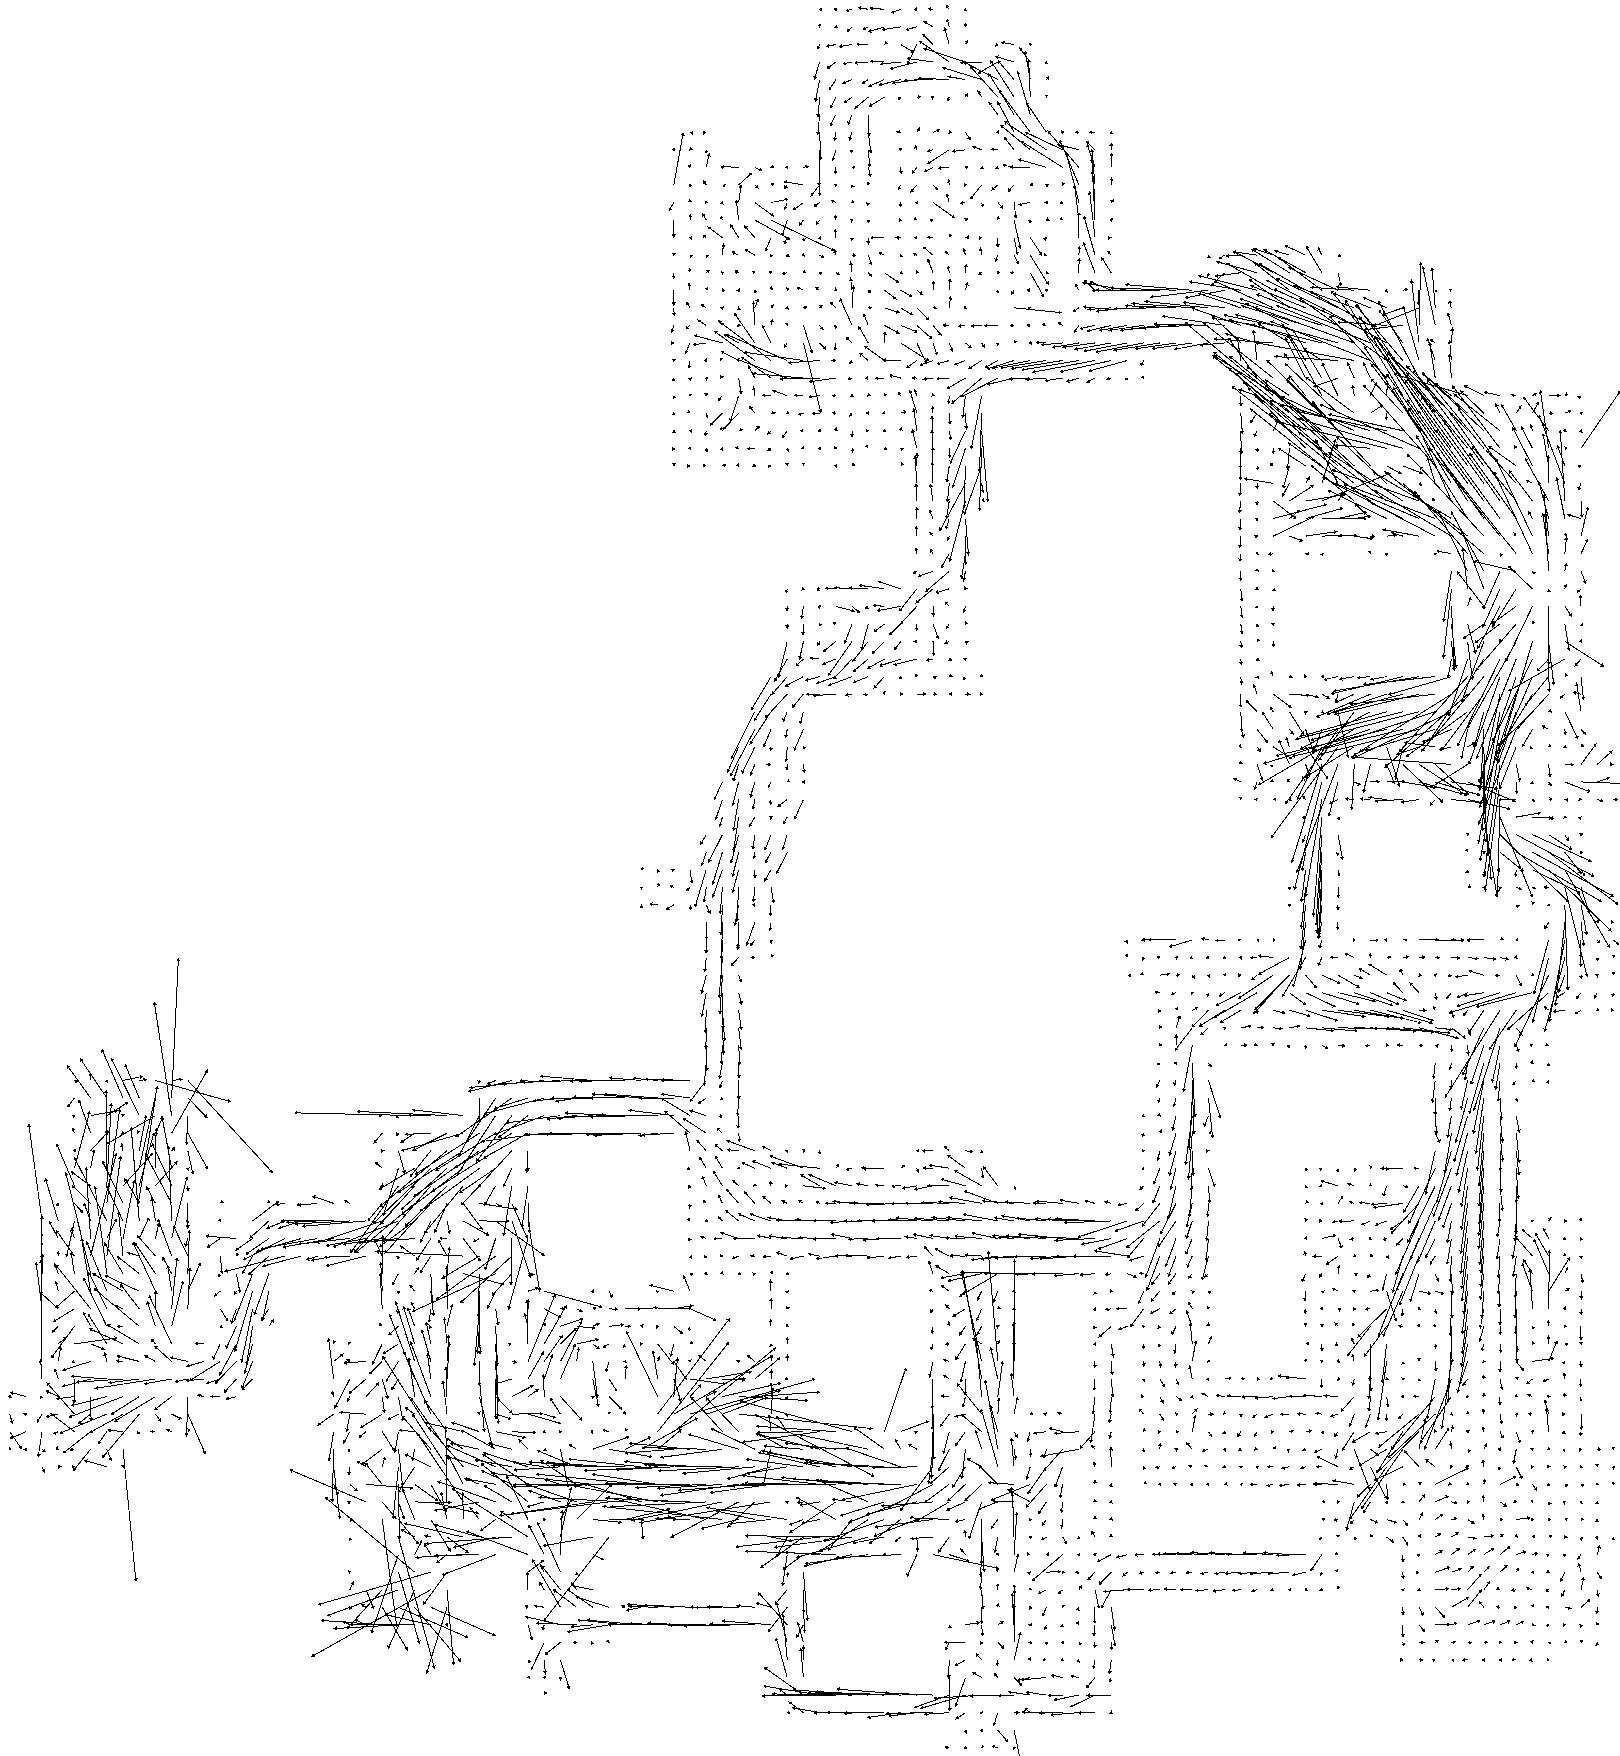
\includegraphics[width=\linewidth]{TrendMapCT.png}
    \caption{The \textit{``CounterTerrorist''} team trend map visually showing stronger trends than the all inclusive trend map shown in fig~\ref{fig:trendmapboth} where the opposing teams meet.}
    \label{fig:trendmap_ct}
\end{figure}

The final stages of development were spent creating the experiment from the previous sprint artefacts. When executed, the program will select at random one path file from the viable data set to be an experiment subject. The remainder are used to create a velocity trend data structure that does not include the chosen experiment subject path to avoid influencing the trend data towards the experiment subject. Once created, a simulation of the chosen path will advance frame by frame with both a standard dead reckoned simulation as described in \ref{deadReckoning}, and this paper's proposed simulation method using the trend data as described in \ref{proposedsolution}, each executing a client-side prediction style simulation upon the data of the chosen path independently of each other. Upon the experiment subject's path completion, each prediction method will return the mean average distance of its own simulation model from the experiment subject's position checked every frame, and the total number of simulated packet updates required. A record of the path length in time is stored alongside these results to calculate the prompted updates per second, and information from CS:GO unit scale conversion rates\footnote[7]{Available: \url{https://developer.valvesoftware.com/wiki/Dimensions}} is used to convert in game measurement units to centimetres for contextual consideration.

For the proposed led reckoned approach to be relevant and comparable to the dead reckoned approach, the proposed variable changes must be relative in value, such that the dead reckoning fixed threshold value is the median value of the range of threshold values for the led reckoning method.

In initial testing of this approach, it became apparent that the zeroing effect of paths travelling in opposite directions to each other, such as up and down a corridor, as suggested in \ref{representingLevelData} was a diminishing factor in the strength of the trends found. Apparent as strong trends found at each team's start location, and a weak trend found where the teams would meet towards the the middle of the map as seen in fig~\ref{fig:trendmapboth}. Consequentially, this project introduces a final filter; that the trend map be constructed only from player paths who belong to the experiment subject's team, and results in the far stronger trend maps shown in fig~\ref{fig:trendmap_t} and fig~\ref{fig:trendmap_ct}. This is justified by the game rules strictly specifying that each team will always start from the same location and have the same team specific goal. To be applied for a general case, we do not have to specify this goal, but accept that by the game's rules it is a constant per team. 

% Previous trend map positions

This filtering is a further refinement of the data set that anticipates future work beyond the scope of this project. We hope that further refinement will be able to discern what other player information is critical to finding strong trends in group behaviour. This may include discerning between players with high and low health amounts, or between those using weapons with long or short ranges. This approach will ultimately borrow from player behaviour modelling so falls beyond this project's reliance upon facts about the player's behaviour which in this case, are the location that they start moving from and the direction of their objective. The author acknowledges that this may not be applicable to other games, but instead refinement factors should be dependant upon behaviour altering constants specific to that game's rules.

\subsection{Software testing} \label{softwaretesting}

Firstly, to test that the prediction algorithms extrapolated correct future positions from movement data, two sets of control data were created to represent two simple cases; zero velocity movement and continuous velocity movement. Algorithm~\ref{algo:test} shows how after a typical experiment is performed, if a test is triggered, the results of that experiment are compared to known control data results. Zero velocity input should return a zero velocity prediction for both prediction methods, and movement with a continuous velocity will return prediction paths that adhere to equation~(1) as shown in fig~\ref{fig:dr1}. For ease, this is movement along a single axis at a constant velocity, so that the results can be manually calculated. All other equations are inferred as working correctly through inheritance given that the experiment program can successfully pass these tests. By implication .NET framework's StreamReader and StreamWriter classes are also tested. Despite being of industry standard quality and established to be reliable, this experiment reads vast quantities of data in a short time which may provoke errors. Example MessageBox user feedback can be seen in fig~\ref{fig:testzero} and fig~\ref{fig:testconstant}.

A third test was introduced to maintain consistency through the iterative development process when optimising, refactoring, or working on visualisation techniques. Three default paths were chosen as control data, where the first acts as the experiment subject path, the second is trend data where the team matches the experiment subject's team, and the third is trend data where the team does not match the experiment subject's team. These paths are suitably complex and the results of this experiment are compared to a previous results file thus indicating consistency.

Regarding the validity of the DEM files, much of the testing was performed with a visual assessment in the GUI. Originally, 164 DEM files were sourced. However, parsing and visualising the data indicated that three of the files were incorrectly listed as the Inferno map. This was visually apparent when the trend was viewed and a safeguard to check the data file for the map name was put in place to check that the DEM replay level is Inferno.

\hrulefill

{\sc Testing using control data pseudo code}

\hrulefill

\begin{algorithm}
\DontPrintSemicolon % Some LaTeX compilers require you to use \dontprintsemicolon instead
\KwIn{ \\
path files: $F_p$ \\
correct results: $R_t$}
$R_p \gets$ \textbf{experiment}($F_p$) \\
\If{is testing}{
    \textbf{Assert}($R_p = R_t$) \\
}
\caption{When testing, control files are passed into the experiment and the results are asserted to be equal to the correct results.}
\label{algo:test}
\end{algorithm}

\section{Results analysis} \label{resultsanalysis}

The experiment was completed 500 distinct times using .NET framework's Random class to choose experiment subjects from the data set of 43,305 paths. In each experiment, the remainder of the data set is used to create the trend data. This paper first examines the results considering each hypothesis detailed in table~\ref{table:hypothesis} before discussing the findings and exploring the implications.

\begin{figure}[h]
    \centering
    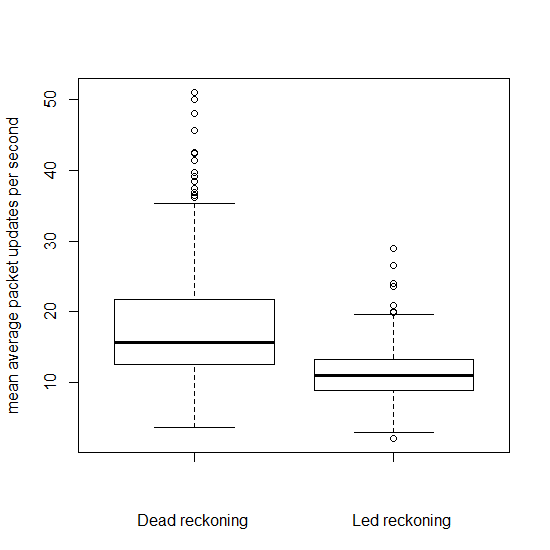
\includegraphics[width=\linewidth]{FinalBoxplotPackets.png}
    \caption{Box plot of the mean average number of prompted packet updates per second for each method.}
    \label{fig:boxplotupdates}
\end{figure}

\begin{figure}[h]
    \centering
    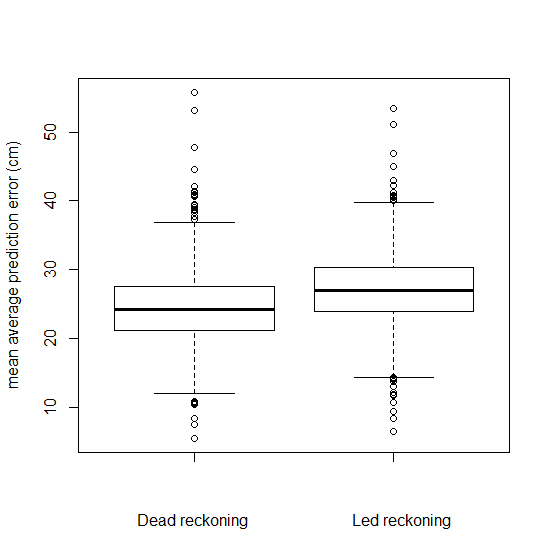
\includegraphics[width=\linewidth]{FinalBoxPlotPosition.png}
    \caption{Box plot of the mean average predicted position error for each method.}
    \label{fig:boxplotdistance}
\end{figure}

\begin{table*}[t]
	\centering
	\caption{Packet update analysis}
	\label{table:resultsupdates}
	\def\arraystretch{1.5}
	\begin{tabular}{|p{2.0cm}p{1.5cm}p{2.5cm}p{1.8cm}p{1.8cm}p{1.8cm}p{1.8cm}|}
		\hline
		& \textbf{Mean}
		& \textbf{Standard deviation}
		& \textbf{\textit{t}-value}
		& \textbf{\textit{df}}
		& \textbf{\textit{p}-value}
		& \textbf{\textit{d}-effect} \\ \hline
		%
		\textbf{Dead reckoning}
		& 17.83246
		& 7.723068
		&  
		&  
		& 
		&  \\
		%
		\textbf{Led reckoning}
		& 11.22664
		& 3.572331
		& 17.359
		& 703.18
		& 2.2 $\times$ 10^{-16} 
		& 1.097877 \\ \hline
	\end{tabular}
\end{table*}

\begin{table*}[t]
	\centering
	\caption{Prediction error analysis}
	\label{table:resultsaccuracy}
	\def\arraystretch{1.5}
	\begin{tabular}{|p{2.0cm}p{1.5cm}p{2.5cm}p{1.8cm}p{1.8cm}p{1.8cm}p{1.8cm}|}
		\hline
		& \textbf{Mean}
		& \textbf{Standard deviation}
		& \textbf{\textit{t}-value}
		& \textbf{\textit{df}}
		& \textbf{\textit{p}-value}
		& \textbf{\textit{d}-effect} \\ \hline
		%
		\textbf{Dead reckoning}
		& 24.79921 
		& 6.36178
		&  
		&  
		& 
		&  \\
		%
		\textbf{Led reckoning}
		& 27.22430  
		& 5.993485
		& -6.2041
		& 994.47
		& 8.057 \times 10^{-10} 
		& 0.392385 \\ \hline
	\end{tabular}
\end{table*}

\subsection{Client-side prediction methods using led reckoning prompt fewer packet updates than those using dead reckoning}

As shown in fig~\ref{fig:boxplotupdates}, the led reckoning method prompts generally far fewer updates per second than the dead reckoning method. The results in table~\ref{table:resultsupdates} show that the mean average number of packet updates prompted by the led reckoning method is 63\% of the mean average number of packet updates prompted by the dead reckoning method. The Cohen's \textit{d}-effect value being greater than one, meaning that the difference in means is larger than one standard deviation, points to a large effect size \cite{cohen2013statistical}. This shows a large improvement and indicates that using led reckoning will significantly reduce network congestion due to a large number of packet updates.

Fig~\ref{fig:boxplotupdates} also shows a much smaller range of packet update rates using led reckoning, with the maximum value for the dead reckoning method nearly double that of the led reckoning method. This maximum value represents a worst case scenario that the network may have to endure, so by decreasing the impact of outlying scenarios, the prediction model can improve the robustness of the network with the most expensive simulations as well as the overall efficiency.

\subsection{Client-side prediction methods using led reckoning are not less accurate than those using dead reckoning} \label{resultsaccuracy}

As shown in fig~\ref{fig:boxplotdistance}, the mean average prediction error that led reckoning methods result in is higher than dead reckoning methods. Despite offering a visually similar range of values, table~\ref{table:resultsaccuracy} shows that the mean average position error of the led reckoning prediction method is 9\% more than that of the dead reckoning method. The \textit{p}-value calculated at considerably less than 0.05 shows that this is statistically significant, rejecting the hypothesis that the accuracy of the prediction remains unchanged described in table \ref{table:hypothesis}. The Cohen's \textit{d}-effect value of 0.392385 shows a small to medium effect size \cite{cohen2013statistical}, which is greater than a sensitivity statistical power analysis using the statistical power calculation program G*Power\footnote[8]{Available: \url{http://www.gpower.hhu.de/}} prescribes at 0.228208 for a two tailed t-test with 500 samples.

\section{Discussion} \label{resultsdiscussion}

Networked multiplayer first-person shooter games use client-side prediction as a tool to help solve the problems associated with latency and packet loss, accepting a trade off between decreasing the amount of network congestion against the cost of decreasing the accuracy of the game state representation for players. To improve upon current client-side prediction methods, either the accuracy of the prediction model, or the required number of packet updates must be improved.

This paper proposes the method led reckoning, which amends the de facto dead reckoning method to include experiential data of previous player routes through a specific level. By comparing the path prediction based on the last known player's actions described in the most recent packet update, against the movement trend for the player's location in game, led reckoning scores the correlation of the prediction to the trend data. This correlation score is used to dynamically adjust the error threshold of the client-side prediction algorithm directly responsible for prompting packet updates, and the time given for the prediction model to reconcile with a new packet's information. Led reckoning considers the trend data as a description of predictable movement, with the supposition that a player acting predictably will continue to act predictably.

Led reckoning is shown to greatly decrease the number of required packet updates by a mean average of 37\% at the cost of increasing the error in position of the prediction algorithm by 9\%. As shown in tables \ref{table:resultsupdates} and \ref{table:resultsaccuracy}, and inherent of large numbers of results, the \textit{p}-values are extremely low, rejecting any null hypothesis of receiving incorrect results. Despite the statistics in \ref{resultsaccuracy} rejecting the hypothesis presented regarding not significantly altering the prediction model's accuracy, this paper must consider the effect size regarding the context of the trade off that client-side prediction presents, in order to evaluate led reckoning's effectiveness.

The increased mean average error is $2.4$cm, calculated from a value of $1.27$ of in game units, and the in game unit conversion of $1$ unit representing $1.905$cm. The experiment uses a constant error threshold for the dead reckoning method of $20$ units or $38.1$cm, and the led reckoning method uses a range of error thresholds from $5$ to $35$ units, or $9.5$cm to $66.7$cm (as outlined in \ref{lifecycle}, the dead reckoning method's constant value acts as the median value of the led reckoning range to be relevant). A developer choosing whether to use led reckoning over dead reckoning must decide if this cost is worth the improvement. The author argues that by considering these expected values of variance, an additional $2.4$cm is minor, and that an effect size of 37\% with network congestion is greater than the effect size cost of 9\% in accuracy.

This discussion must also acknowledge a fundamental factor omitted from the experiment, that of the effects of network congestion. As mentioned in \ref{discussion}, late or lost packets caused by network congestion have a severe impact upon the simulation. This project omitted any simulation of network congestion effects within the experiment which would undoubtedly have a negative impact upon the accuracy of the prediction methods. Were a packet update prompted by excessive prediction error not to be received, then the prediction method relying upon that packet update would continue upon its erroneous path. It is reasonable to assume that with more packet updates late or lost, the reliant prediction method would become more error prone; ergo, the dead reckoning method shown to incur higher network congestion cost than the led reckoning method will be more error prone. Without the experiment including simulated packet congestion, conjecture upon the effect of increased late or lost packets is unable to state whether the difference in accuracy of the dead reckoning method over the led reckoning method would be negated. But, in examining the implications of decreasing network congestion, it is reasonable to state that the mean average accuracy of the prediction simulation would be improved.

The evidence shown by the results of the experiment suggest that led reckoning is a valid alternative to dead reckoning given that there is opportunity to collect experiential data upon relatable player paths beforehand. The improvements shown by using this method will directly benefit the player's of the game who suffer from poor game state management due to over congested network traffic, and the developers of the game whose hard work is often overlooked due to client dissatisfaction with network performance.

In implementation, the trend data should be computed during the game's development and packaged with the level. As discussed in appendix~\ref{app:factors}, multiple trend maps could be packaged with a level each filtered by a different trait. Led reckoning would then choose the most appropriate trend data to use, based upon the player state.

\section{Limitations} \label{limitations}

As with any experiment based upon finding trends within data, this experiment is limited by the variation in the sourced data set. The trend data is formed from skilled player's playing under tournament conditions justified as seeking the \textit{best} paths. But in actuality, this is potentially fixing the results to only work for similarly skilled players. Further experimentation is needed to see if these trends are transferable between skill levels. This project must consider that by definition highly skilled players will play the game in a different way to lower skilled players.

This method of deriving a set of trend data is only applicable to a static level. Games can often introduce dynamic or destructible elements to the level which will affect the paths of players. These can be in the form of destructible buildings or scenery, possibly concealing or revealing future route options through the level. Props such as vehicles can often be moved to obstruct or allow access to an area of the map, and these vehicles will often adhere to different movement rules. Players may also have access to traps or barriers within their inventory, whose presence within the level will deter player's from a particular path.

Finally, we cannot say if this method works for every map, we can only say that the evidence suggests that this method works in this way for CS:GO's Inferno map. Considerable testing will need undertaking before this can be seen as a broadly applicable method.

\section{Future work} \label{futurework}

The effects of network congestion upon the prediction methods must be explored given that led reckoning is shown to decrease this factor at the cost of accuracy. As discussed in \ref{resultsdiscussion}, the implications of network congestion may improve or negate the slight change in prediction accuracy but this must be investigated. By incorporating network simulation into future work this, and other potential network simulation factors such as jitter or latency, can be explored.

Led reckoning has been shown to work as a proof of concept for a level that can be represented as a two dimensional data structure. Future work should recreate this process with a multilevel map as shown in fig~\ref{fig:hm2}. Other than restructuring the data structures, the author suggests if factoring in verticality, different possible movement mechanics such as jumping and falling may need to be considered.

As noted in \ref{limitations}, this method is currently only shown to work for Inferno. Future work should test led reckoning on many different game maps, which is straightforward given the abundance of CS:GO replay data available. If shown to be effective with CS:GO for a general case, then other games should be considered next. This should not be limited to first-person shooter games, but include any game where dead reckoning is used to maintain an up to date game state representation while minimising network traffic. This should include racing games and sports games.

Lastly, other than generating the trend data repeatedly, there is currently no method for the trend data to receive new data. The author proposes that this offers the most promising direction for the field, as given a base trend map offering initial guidance for the led reckoning algorithm to follow, the trend data would be able to accumulate and accommodate paths preferable for its own specific player. This would build a specific trend model based on that player's experience within the map which the author proposes will result in a far more probable representation of likely paths throughout. Similar to Yahyavi \textit{et al}'s method, attraction forces may be factored into the equation of motion to tend the prediction model towards a path that is influenced by that specific player's previous experience.

\section{Conclusion}

Research into client-side prediction methods seek to improve either the number of required packet updates or the accuracy of the prediction model. The literature review shows that this can be achieved with potentially expensive examinations of the game or player state at the prediction time. To the authors knowledge, no research exists on using precalculated data to influence the client-side prediction algorithm.

The described led reckoning method uses movement trends found from examining previous player paths through the level to influence the packet update conditions of the client-side prediction algorithm resulting in a large reduction of the range and required number of packet updates, at the cost of a small increase in prediction error. This small effect on prediction error may be further reduced when the implications of a less congested network are exhibited.

In this study the trend data has been filtered by team to offer trend data more relevant to the modelled agent's future actions. Further filtering is acknowledged as potentially valuable, although understanding a player's motivation to better predict future actions falls beyond the scope of this study. Given the small size of the processed trend data, many trends may be packaged with a level relating to differing player or game states which may influence future actions.

% references section

\bibliographystyle{IEEEtran}
\bibliography{references}

% Appendices

\appendices
\section{Acknowledgements}

I would like to thank my project supervisor Gareth Lewis whose guidance, patience, and fruitful discussions have been invaluable to this body of work. I would also like to thank all of the staff at Falmouth University Games Academy as they have all at some point been subject to my questions and have been endlessly patient and helpful in response.

\section{Reflective report}

This paper proposes promising amendments to dead reckoning based client-side prediction methods, and I am proud of its finished state. However, it uses only a small amount of the information available, which I'm sure if given proper consideration would yield better results. My time was instead largely spent trying to refine parsing the intimidatingly large data set. An obvious acknowledgement of my initial poor choices in approach indicating a lack of experience.

\subsection{Large amounts of data} \label{databaseapproach}

This project attempted many different methods to deal with having a large data set. The first successful method used an SQLite database to hold all 85,000,000 rows of frame data. However, querying that database 10,000 times (for a $100 \times 100$ data structure) would take more than twenty hours to complete. It was at this point that I discovered the rogue non-Inferno level data contamination (mentioned in \ref{softwaretesting}) and resignedly faced having to run the program again. Even populating the database was a daunting task with so many entries to add. However, this became an opportunity to learn more about databases and I now know how to commit large SQLite transactions in bulk commits.

Eventually, I reexamined the use case of the data and realised that the experiment did not need the accumulated data in one perpetual file. Instead, the proposed method uses a file stream reader and loads the data sequentially into memory, processing it line by line. This was an arduous task still and took some effort to optimise into a sensible use time which now requires around two minutes to complete. An attempt to rewrite and optimise the process in the potentially more efficient language C++ showed no discernible improvement in efficiency. Although, the I concede that this may be due to a lack of experience with the tool.

Following this project, I will complete the Pluralsight SQLite courses\footnote[9]{Available: \url{https://app.pluralsight.com/search/?q=sqlite}} so that I better understand the use cases of my initial database driven method over the approach ultimately used by this project. I recommend that anyone planning on using very large amounts of data consider how they will be using that data before researching appropriate methods.

\subsection{Acceleration adjustment}

This project began with an attempt to use the velocity trend data to influence the acceleration factor similar to Yahyavi \textit{et al}'s method described in \ref{interestModelling}. In hindsight, I stubbornly held on to the belief that this was a potential result of using the trend data for too long. Perhaps this approach is worthwhile, but I believe this will need to consider modelling player motivation which this project has sought to avoid.

Before continuing with this research I must learn more about modelling player motivation. Due to Yahyavi \textit{et al}'s success, I will read all of the scientific papers that their paper cites to better understand the reasoning behind their method and its success. I recommend researching player behaviour to anyone who is studying the field of client-side prediction.

\subsection{Testing with non-professional data}

While using existing replay data has yielded a large amount of research data, the experiment subjects have been of the same ilk; highly skilled CS:GO players. This method cannot be considered a general approach for improvement until it can be shown to be effective for players of all skills. Where this project's experiment subjects will likely be playing effectively towards the objective, often taking the most efficient route across the level, I must consider how well this method will predict less predictable behaviour for example of a player with no experience of the level. I would hope that even the least experienced player would move up and down a corridor, rather than moving directly into a barrier, but this requires relevant replay data to test.

We must also consider that by originating from gameplay potentially marred by poor client-side prediction, the data set may already be contaminated. Until able to train the data set on conclusively reliable data there remains the possibility that the data set may contain player's that are inherently behaving differently than normal because of previous client-side prediction error. This is difficult to account for given the current data source.

Also, practically for real world use, this method will need testing in a real time setting before recommending its general use. The effects of jitter, network latency, and packet loss have been conveniently omitted with the focus upon update frequency, but yet are still acknowledged as the motivation for this work. I predict that these potentially strenuous settings will further reveal the potential of using experiential data to influence client-side prediction methods. Exploring these use case scenario complications is paramount to any subsequent research into this field.

\subsection{Alternate factors} \label{app:factors}

Given the small size of the trend data, many specific case trends could be packaged with a level to be used and swapped between depending on the player's situation. Similar to filtering the trend forming input data by team name, any of the variables listed in \ref{lifecycle} could be equally or more effective. Considering that a player will often move laterally, longitudinally, or along a diagonal vector between these, relative to the player's facing direction as the keyboard controls of CS:GO dictate, it follows that the view direction may arguably be very important. Similarly, the current weapon, the score of the game, or the agent's health amount, all offer significant value as a movement changing motivator. As acknowledged in \ref{lifecycle} and \ref{futurework}, the team filtering is the start of what I consider as future work in the field, and any future work by myself or others should explore at least one other potential factor.

\subsection{Conclusion}

As a self-directed project, I am thrilled by the results shown from the experiment. I wanted to concentrate upon the mathematics theory of the algorithms rather than player modelling, and have mostly maintained this approach although have surmised that future research must include player behaviour modelling consideration. Sourcing the movement data from online reputable sources has saved me a large amount of time in creating a test bed then recruiting participants to play it, allowing the easy collection of a far greater amount of data than I could hope to collect in person given the project's scope. I have also greatly enjoyed the discussion in trade off between the accuracy and number of packets as a challenge that would not have been available had both of my hypotheses been initially confirmed. This required careful thought and scrutiny about what client-side prediction entails, what it achieves, and how it might be improved. \\ \\

\section{Additional materials}

\subsection{Quality assurance}

\begin{figure}[h]
    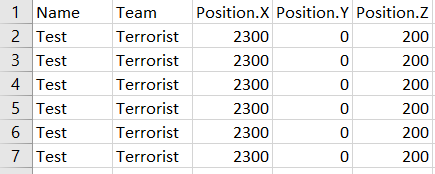
\includegraphics[width=0.7\linewidth]{TestZeroVelocityRawData.png}
    \caption{A portion of the manually written zero velocity control data}
\end{figure}

\begin{figure}[h]
    \centering
    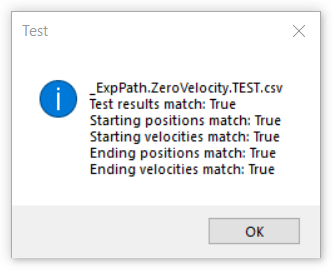
\includegraphics[width=0.7\linewidth]{TestZero.png}
    \caption{Example feedback from a zero velocity control data test showing the experiment results matching and individual variable test cases matching across the parsed data file and both prediction methods.}
    \label{fig:testzero}
\end{figure}

\begin{figure}[h]
    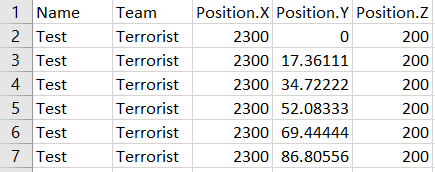
\includegraphics[width=0.7\linewidth]{TestConstantVelocityRawData.png}
    \caption{A portion of the manually written and calculated constant velocity control data. This was manually calculated using Newton's laws of motion.}
\end{figure}

\begin{figure}[h]
    \centering
    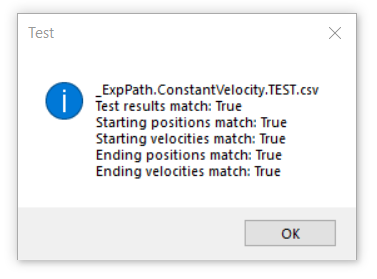
\includegraphics[width=0.7\linewidth]{TestConstant.png}
    \caption{Example feedback from a constant velocity control data test showing the experiment results matching and individual variable test cases matching across the parsed data file and both prediction methods.}
    \label{fig:testconstant}
\end{figure}

% that's all folks
\end{document}